% Options for packages loaded elsewhere
\PassOptionsToPackage{unicode}{hyperref}
\PassOptionsToPackage{hyphens}{url}
%
\documentclass[
  11pt,
]{article}
\usepackage{lmodern}
\usepackage{amssymb,amsmath}
\usepackage{ifxetex,ifluatex}
\ifnum 0\ifxetex 1\fi\ifluatex 1\fi=0 % if pdftex
  \usepackage[T1]{fontenc}
  \usepackage[utf8]{inputenc}
  \usepackage{textcomp} % provide euro and other symbols
\else % if luatex or xetex
  \usepackage{unicode-math}
  \defaultfontfeatures{Scale=MatchLowercase}
  \defaultfontfeatures[\rmfamily]{Ligatures=TeX,Scale=1}
\fi
% Use upquote if available, for straight quotes in verbatim environments
\IfFileExists{upquote.sty}{\usepackage{upquote}}{}
\IfFileExists{microtype.sty}{% use microtype if available
  \usepackage[]{microtype}
  \UseMicrotypeSet[protrusion]{basicmath} % disable protrusion for tt fonts
}{}
\makeatletter
\@ifundefined{KOMAClassName}{% if non-KOMA class
  \IfFileExists{parskip.sty}{%
    \usepackage{parskip}
  }{% else
    \setlength{\parindent}{0pt}
    \setlength{\parskip}{6pt plus 2pt minus 1pt}}
}{% if KOMA class
  \KOMAoptions{parskip=half}}
\makeatother
\usepackage{xcolor}
\IfFileExists{xurl.sty}{\usepackage{xurl}}{} % add URL line breaks if available
\IfFileExists{bookmark.sty}{\usepackage{bookmark}}{\usepackage{hyperref}}
\hypersetup{
  pdftitle={Evolution along allometric lines of least resistance: Morphological differentiation in Pristurus geckos},
  hidelinks,
  pdfcreator={LaTeX via pandoc}}
\urlstyle{same} % disable monospaced font for URLs
\usepackage[margin=1in]{geometry}
\usepackage{graphicx,grffile}
\makeatletter
\def\maxwidth{\ifdim\Gin@nat@width>\linewidth\linewidth\else\Gin@nat@width\fi}
\def\maxheight{\ifdim\Gin@nat@height>\textheight\textheight\else\Gin@nat@height\fi}
\makeatother
% Scale images if necessary, so that they will not overflow the page
% margins by default, and it is still possible to overwrite the defaults
% using explicit options in \includegraphics[width, height, ...]{}
\setkeys{Gin}{width=\maxwidth,height=\maxheight,keepaspectratio}
% Set default figure placement to htbp
\makeatletter
\def\fps@figure{htbp}
\makeatother
\setlength{\emergencystretch}{3em} % prevent overfull lines
\providecommand{\tightlist}{%
  \setlength{\itemsep}{0pt}\setlength{\parskip}{0pt}}
\setcounter{secnumdepth}{-\maxdimen} % remove section numbering
\usepackage{setspace}\doublespacing
\usepackage{lineno}\linenumbers
\usepackage[utf8]{inputenc}
\usepackage[T1]{fontenc}
\usepackage{biblatex}
\usepackage{booktabs}
\usepackage{longtable}
\usepackage{array}
\usepackage{multirow}
\usepackage{wrapfig}
\usepackage{float}
\usepackage{colortbl}
\usepackage{pdflscape}
\usepackage{tabu}
\usepackage{threeparttable}
\usepackage{threeparttablex}
\usepackage[normalem]{ulem}
\usepackage{makecell}
\usepackage{xcolor}

\title{Evolution along allometric lines of least resistance: Morphological
differentiation in \emph{Pristurus} geckos}
\author{}
\date{\vspace{-2.5em}}

\begin{document}
\maketitle

\begin{center}
\textbf{H{\'{e}}ctor Tejero-Cicu{\'{e}}ndez$^{1,2,*}$,  Iris Men{\'{e}}ndez$^{3}$, Adri{\'{a}}n Talavera$^{2}$, Gabriel Riaño$^{2}$, Bernat Burriel-Carranza$^{2}$, Marc Sim{\'{o}}-Riudalbas$^{2}$, Salvador Carranza$^{2}$, and Dean C. Adams$^{4}$}
\end{center}

\begin{center}19 enero, 2023\end{center}

\(^{1}\)Evolution and Conservation Biology research Group, Department of
Biodiversity, Ecology and Evolution. Faculty of Biology. Universidad
Complutense de Madrid, 28040, Madrid, Spain

\(^{2}\)Institute of Evolutionary Biology (CSIC-Universitat Pompeu
Fabra), Passeig Marítim de la Barceloneta 37-49, Barcelona 08003, Spain

\(^{3}\)Museum für Naturkunde, Leibniz Institute for Evolution and
Biodiversity Science, Berlin, Germany

\(^{4}\)Department of Ecology, Evolution, and Organismal Biology, Iowa
State University, Ames, Iowa, 50010 USA

\(^{*}\)Correspondence: Héctor Tejero-Cicuéndez
\href{mailto:cicuendez93@gmail.com}{\nolinkurl{cicuendez93@gmail.com}}

\newpage

\hypertarget{abstract}{%
\section{Abstract}\label{abstract}}

Species living in distinct habitats often experience unique ecological
selective pressures, which can drive phenotypic divergence. However, how
ecophenotypic patterns are affected by allometric trends and trait
integration levels is less well understood. Here we evaluate the role of
allometry in shaping body size and shape diversity in \emph{Pristurus}
geckos utilizing differing habitats. We found that patterns of body
shape allometry and integration were distinct in species with different
habitat preferences, with ground-dwelling \emph{Pristurus} displaying
the most divergent allometric trend and the strongest integration. There
was also strong concordance between static allometry across individuals
and evolutionary allometry among species, revealing that body shape
differences among individuals were predictive of evolutionary changes
across the phylogeny at macroevolutionary scales. This suggested that
phenotypic evolution occurred along allometric lines of least
resistance, with allometric trajectories imposing a strong influence on
the magnitude and direction of size and shape changes across the
phylogeny. When viewed in phylomorphospace, the largest rock-dwelling
species were most similar in body shape to the smallest ground-dwelling
species, and vice versa. Thus, in \emph{Pristurus}, phenotypic evolution
along the differing habitat-based allometric trajectories resulted in
similar body shapes at differing body sizes in distinct ecological
habitats.

\newpage

\hypertarget{introduction}{%
\section{1. Introduction}\label{introduction}}

Understanding how phenotypic diversity evolves, and elucidating the
forces that generate and maintain this diversity, are major goals in
evolutionary biology. Because adaptive evolution is the product of
natural selection, changes in ecological selection pressures are
expected to affect the evolutionary trajectory of phenotypic traits that
facilitate an organism's survival in their habitat. Evolutionary theory
predicts that differing habitats will exert unique ecological selection
pressures on organisms, resulting in associations between ecological and
phenotypic traits. Indeed, species inhabiting differing habitats often
display functional, behavioral, or phenotypic differences, that have
presumably been the result of adaptive diversification in their
respective ecological contexts (Collar et al. 2010; Kaliontzopoulou et
al. 2015; Price et al. 2015; Martinez et al. 2021; Kolmann et al. 2022).
\hfill\break

One possible evolutionary outcome of ecological specialization is that
organisms inhabiting similar environments display common phenotypic
characteristics. When such patterns occur repeatedly (Losos 1992;
Schluter and McPhail 1992), this convergent evolution is treated as
strong evidence of adaptation. Indeed the ecomorphological paradigm
(Arnold 1983) is predicated, in part, on such cases, which emphasize the
strong association between the phenotypic traits that organisms display
(morphological, behavioral, or physiological) and the ecological
characteristics of their habitat that mediate organismal performance. In
vertebrates, ecomorphological trends have been well studied in numerous
taxonomic groups, and include the emblematic `ecomorphs' of Caribbean
\emph{Anolis} lizards that exploit different microhabitats (Losos 1992,
2009; Mahler et al. 2013), differential beak morphology in species of
Darwin's finches (Schluter and Grant 1984; Grant and Grant 2006; Reaney
et al. 2020), the recurring phenotypes of African lake cichlids across
ecological regimes (Albertson and Kocher 2001; Urban et al. 2022), and
the distinct body forms of freshwater fishes in benthic and limnetic
habitats (Jastrebski and Robinson 2004; Berner et al. 2008; Stuart et
al. 2017), among others. \hfill\break

However, while the patterns of morphological differences in distinct
ecological contexts have been well documented, less-well understood is
how this differentiation has been influenced by trait covariation
associated with body size differences (i.e., allometry). Evaluating
allometric trends across hierarchical levels (e.g., comparing allometry
at the individual level, or static allometry, and among species, or
evolutionary allometry) may aid in our understanding of how adaptive
morphological change occurs at macroevolutionary scales (Klingenberg and
Zimmermann 1992). It has long been recognized that the
interrelationships among traits can exert a strong influence on how
phenotypic evolution proceeds, as trait correlations influence the
degree to which phenotypic variation is exposed to selection (Wagner and
Altenberg 1996). Thus, the integration among traits can constrain
phenotypic change in certain directions, or enhance variation along
other phenotypic axes (Schluter 1996; Wagner and Altenberg 1996; Wagner
and Zhang 2011; Klingenberg and Marugán-Lobón 2013; Goswami et al. 2014,
2016; Felice et al. 2018; Navalón et al. 2020). Further, because nearly
all linear traits covary strongly with overall body size (Jolicoeur
1963; Bookstein 2022), allometric trends could be considered the
quintessential expression of phenotypic integration. Thus, identifying
whether allometric patterns differ across habitats, and how such
patterns of trait covariation affect ecomorphological trends among
species utilizing those habitats, remains an important question worthy
of investigation. \hfill\break

The Afro-Arabian geckos in the genus \emph{Pristurus} afford the
opportunity to elucidate the interdigitating effects of allometry and
habitat specialization on clade-level patterns of phenotypic diversity.
Prior work on this system (Tejero-Cicuéndez et al. 2021a) revealed that
the colonization of ground habitats has been a trigger of morphological
change, specifically reflected in an increase in body size and shape
disparity. Interestingly, some ground-dwelling species are among the
largest of the genus and also show increased relative head sizes and
limb proportions, while some other species with this ecological
specialization have evolved to be among the smallest of the group.
Additionally, among the species exploiting rocky habitats (the most
common ecological feature in \emph{Pristurus}), there are also species
with both considerably large and small body sizes (Tejero-Cicuéndez et
al. 2021a). What remains unexplored, however, is how the evolution of
body shape is related to differences in body size and whether habitat
specialization has an impact in this shape-size relationship.
\hfill\break

In this study, we employed a combination of multivariate morphometric
and phylogenetic comparative analyses to interrogate macroevolutionary
patterns of evolutionary allometry in \emph{Pristurus} geckos of
Afro-Arabia. Using phenotypic, phylogenetic, and ecological data, we
first characterized allometric trends in body form in the group, to
discern the extent to which evolutionary allometric trends across the
phylogeny aligned with habitat-based static allometry for species
occupying distinct ecological regimes. We then examined changes in
allometric trends across the phylogeny, and linked these patterns to
overall phenotypic integration, diversification in morphospace, and
habitat utilization among taxa. Our analyses reveal that patterns of
evolutionary allometry across species align with allometric trends
within habitats, demonstrating that the interplay between ecological
specialization and allometric trajectories in species with disparate
body size may play a determinant role in shaping the phenotypic
evolution and hence in adaptive dynamics in this clade.

\hypertarget{materials-and-methods}{%
\section{2. Materials and Methods}\label{materials-and-methods}}

\hypertarget{a-data}{%
\subsection{(a) Data}\label{a-data}}

We used a combination of phenotypic, phylogenetic, and ecological data
to characterize and evaluate intra- and interspecific allometric trends.
The data utilized here were obtained from our prior work on this system
(Tejero-Cicuéndez et al. 2021a, 2022), and are briefly described here.
First we used a time-dated, molecular phylogeny of squamates that
included all members of the genus \emph{Pristurus}, including several
currently undescribed taxa. The tree was estimated in a Bayesian
framework, using five mitochondrial markers, six nuclear markers, and 21
calibration points (Tejero-Cicuéndez et al. 2022). Next we categorized
each species as belonging to one of three ecological groups (ground,
rock, or tree), based on descriptions of habitat use found in the
literature (Tejero-Cicuéndez et al. 2021a). Finally, we obtained a
phenotypic data set containing body size (snout-vent length: SVL) and
eight linear measurements (Figure 1) that described overall body form:
trunk length (TL), head length (HL), head width (HW), head height (HH),
humerus length (Lhu), ulna length (Lun), femur length (Lfe), and tibia
length (Ltb) (Tejero-Cicuéndez et al. 2021a). We restricted our study to
those species represented by nine or more individuals; resulting in a
dataset of 687 individuals from 25 species (invidivuals per species:
\(\mu=27\); min = 9, max = 56). Species in the phenotypic dataset were
then matched to the phylogeny, which was subsequently pruned to the
final topology. All measurements were log-transformed prior to
statistical analyses. Additional details regarding data collection and
formal descriptions of each linear measurement may be found in the
original sources (Tejero-Cicuéndez et al. 2021a, 2022). The data are
available on DRYAD: \url{https://doi.org/10.5061/dryad.xwdbrv1f6}
(Tejero-Cicuéndez et al. 2021b).

\hypertarget{b-statistical-and-comparative-analyses}{%
\subsection{(b) Statistical and Comparative
Analyses}\label{b-statistical-and-comparative-analyses}}

We conducted a series of analyses to interrogate allometric trends,
patterns of integration, and macroevolutionary changes in allometry,
relative to differentiation in body form. First we characterized
evolutionary allometry in the genus by performing a phylogenetic
multivariate regression of body form on body size (i.e., SVL), using the
species means as data. We then performed an analogous procedure at the
individual level, regressing body form on body size using our entire
dataset. From both the species-level (phylogenetic) and the
individual-level analyses, we obtained the set of regression
coefficients, and calculated the difference in their angular direction
to describe the extent to which patterns of allometry at the individual
level were concordant with evolutionary allometric trends across
species. \hfill\break

Next we used the dataset containing all individuals to determine whether
trends in static allometry differed across habitat groups. This was
accomplished by performing a multivariate analysis of covariance, with
body size (\(SVL\)), \(habitat\), and \(SVL \times habitat\) as model
effects. Significance was evaluated using 999 iterations of a
permutation procedure, where residuals from a reduced model were
randomly permuted in each permutation (RRPP), model statistics were
recalculated, and used to generate empirical null sampling distributions
to evaluate the observed test statistics (following Freedman and Lane
1983; Collyer and Adams 2007; Collyer et al. 2015). We then compared the
multivariate allometric vectors for each habitat group to one another,
and to a vector representing multivariate isometry, by calculating
pairwise differences in their angular direction in morphospace, and
evaluating these relative to empirical sampling distributions obtained
through RRPP (Collyer and Adams 2007, 2013; Adams and Collyer 2009).
Here, residuals were obtained from a common isometry reduced model,
whose common slope component described a pattern of multivariate
isometry, and whose intercepts allowed for differences in least-squares
means among groups. Patterns of multivariate allometry relative to body
size were visualized via regression scores (Drake and Klingenberg 2008)
and predicted lines (Adams and Nistri 2010), based on the coefficients
and fitted values from the linear model described above. \hfill\break

Additionally, because allometry describes the extent to which traits
covary with body size and with each other (i.e., integration), we
conducted an analysis of integration. Here we characterized the extent
of morphological integration in body form for individuals within each
habitat group by summarizing the dispersion of eigenvalues of their
respective trait covariance matrix (Pavlicev et al. 2009). This measure
(\(V_{rel}\)) was subsequently converted to an effect size (a
\(Z\)-score), which quantified the strength of morphological integration
(Conaway and Adams 2022). We then performed a series of two-sample tests
to compare the strength of morphological integration across habitat
groups, following the procedures of (2022). Additionally and for
comparison, we repeated these analyses on the set of size-standardized
trait data, found as a set of shape ratios (Mosimann 1970) where each
trait was divided by body size (Supplementary Material). \hfill\break

To determine the extent to which static and evolutionary allometry were
concordant, we evaluated the directions in morphospace of both the
evolutionary (species-level) and static (habitat-based) allometric
trends. Specifically, we obtained the set of regression coefficients
from both the phylogenetic multivariate regression and the multivariate
analysis of covariance analyses above, and calculated the differences in
angular direction between the evolutionary trajectory and the static
allometry trend for each habitat group. The observed angles were then
statistically evaluated relative to empirical sampling distributions
obtained through permutation (RRPP), based on the common isometry model
described above. \hfill\break

Next, to discern how allometric trends resulted in the evolution of
distinct body forms, we examined changes in the body shape proportions
across the phylogeny. Here we treated the head dimensions and limb
dimensions separately, as allometric trends could potentially differ
between these body regions due to differential functional or selective
constraints (Kaliontzopoulou et al. 2010). Because both the head and
limb data were multivariate, we first performed a partial least squares
(PLS) analysis (Rohlf and Corti 2000) of the head traits versus SVL, and
the limb traits versus SVL, to describe the direction of maximal
covariation between each body region and size. We then measured the mean
residuals of each species to the inferred allometric trend, which
described the extent to which head and limb proportions of species were
greater or smaller than expected for their body size. The species
residuals were then mapped on the phylogeny of \emph{Pristurus} using a
Brownian motion model of evolution, to qualitatively evaluate shifts in
head and limbs proportionality across the phylogeny for the group.
Similarly, within-species patterns of static allometry were visualized
by plotting regressions of PLS scores on SVL for both head and limb
traits separately. \hfill\break

Finally, to relate within-species allometric trends with patterns of
phenotypic diversification in the group we generated a phylomorphospace,
based on a phylogenetic principal component analyses (PCA) on the
size-standardized species means obtained from a phylogenetic regression
(see Tejero-Cicuéndez et al. 2021a). Here, phenotypic similarities among
species, relative to their phylogenetic relationships and habitat
affiliations, were observed. Additionally, representative specimens
(scaled to unit size) were also visually compared to aid in describing
these trends. A similar phylomorphospace was constructed for species
means not corrected for body size, and the phenotypic disparity among
species means in each habitat was calculated and subsequently compared
(Supplementary Material). All analyses were conducted in R 4.2.1 (R Core
Team 2022), using \texttt{RRPP} version 1.3.1 (Collyer and Adams 2018,
2022) and \texttt{geomorph} 4.0.4 (Baken et al. 2021a) for statistical
analyses and the \texttt{tidyverse} version 1.3.0 (Wickham et al. 2019),
\texttt{phytools} version 0.7-77 (Revell 2012), and a modified version
of the function \texttt{ggphylomorpho}
{[}\url{https://github.com/wabarr/ggphylomorpho}{]} for data
manipulation and visualization, as well as scripts written by the
authors (Supplementary Material).

\hypertarget{results}{%
\section{3. Results}\label{results}}

Using phylogenetic regression, we found significant evolutionary
allometry in body form across species (\(N_{sp}=25\); \(F = 217.9\);
\(Z =5.53\); \(P < 0.001\)). Likewise, when allometry in body form was
examined across individuals, a similar pattern was observed
(\(N_{ind}=687\); \(F = 7910.8\); \(Z =9.20\); \(P < 0.001\)). Further,
the vectors of regression coefficients between the two analyses were
highly correlated (\(\rho = 0.94\)) and were oriented in nearly parallel
directions in morphospace (\(\theta = 1.49^\circ\)). This revealed that
the pattern of multivariate allometry across individuals was concordant
with macroevolutionary trends of interspecific allometry among species
of \emph{Pristurus} across the phylogeny. \hfill\break

Our analyses also exposed significant differences in the allometry of
body form among \emph{Pristurus} utilizing distinct habitats (Table 1).
Further, pairwise comparisons of multivariate allometric vectors
revealed that patterns of static allometry in each habitat differed
significantly from isometry, indicating the presence of multivariate
allometry in each (Table 2). Additionally, comparisons identified that
ground-dwelling \emph{Pristurus} displayed the most distinct allometric
trend as compared with \emph{Pristurus} occupying both the rock and tree
habitats (Table 2; Figure 2). Here, regression coefficients of each
trait versus size (Supplementary Material) revealed that ground-dwelling
\emph{Pristurus} exhibited strong positive allometry for all head and
limb traits (i.e., \(\beta>1.0\)). By contrast, rock and tree-dwelling
\emph{Pristurus} displayed negative allometry (i.e., \(\beta < 1.0\))
for head traits, and were more varied for limb traits; with
rock-dwelling \emph{Pristurus} displaying positive limb allometry
(though less extreme than that of ground-dwelling taxa), whereas most
limb traits in tree-dwelling taxa showed negative allometry or
near-isometry (Supplementary Material). Thus, these findings implied
that larger individuals of ground-dwelling \emph{Pristurus} species
displayed disproportionately larger heads and limbs, as compared with
large individuals in taxa utilizing other habitat types. Multivariate
visualizations of these multivariate allometric trends (Figure 2)
confirmed these statistical findings, and indicated that the allometric
trajectory in ground-dwelling \emph{Pristurus} was more extreme as
compared with either rock- or tree-dwelling \emph{Pristurus}.
\hfill\break

Examination of patterns of trait covariation revealed strong levels of
morphological integration within each habitat type (\(Z_{ground}=3.97\);
\(Z_{rock}=3.72\); \(Z_{tree}=2.15\)). Further, two-sample tests
revealed that the strength of morphological integration was
significantly greater in ground-dwelling \emph{Pristurus} than either
those utilizing rock (\(Z_{ground-rock}=6.59\); \(P << 0.001\)) or tree
habitats (\(Z_{ground-tree}=11.17\); \(P << 0.001\)). Arboreal
\emph{Pristurus} displayed the lowest levels of integration, which were
also significantly lower than in the rock habitat
(\(Z_{rock-tree}=7.19\); \(P << 0.001\)). When size was accounted for in
the data, levels of integration dropped considerably, though the overall
pattern and differences among habitat groups remained the same
(Supplementary Material). \hfill\break

Comparisons of evolutionary allometry with static allometry in each
habitat revealed substantial concordance between allometric trends at
these hierarchical levels. Here, vectors of regression coefficients
representing static allometry within habitat groups were oriented in
very similar directions with the regression vector representing
evolutionary allometry, with small pairwise angles between them
(\(\theta: 2.3^\circ\rightarrow5.9^\circ\)). Subsequent permutation
tests indicated no differences between the static allometry vectors and
the regression vector representing evolutionary allometry, indicating
strong congruence between them (Table 3). Notably, static allometry in
ground-dwelling \emph{Pristurus} was most similar to trends of
evolutionary allometry, displaying the smallest angular difference and
largest effect size. Thus, static and evolutionary allometry trends were
essentially parallel in this group, indicating a direct correspondence
between the two. This result implied that phenotypic evolution across
species aligned closely with directions of allometric variation within
habitat groups at the individual level; namely that larger individuals
and larger ground-dwelling species exhibited disproportionately larger
heads and limbs, while smaller individuals and smaller ground-dwelling
species displayed disproportionately smaller heads and limbs.
\hfill\break

Mapping the residuals of species into the phylogeny showed that large
ground-dwelling species displayed greater head proportions than large
rock-dwelling species, who exhibited smaller heads relative to body size
(Figure 3A). Conversely, the opposite pattern was observed when
comparing small species utilizing these habitats: ground-dwelling
species showed small relative head proportions while rock-dwelling
species displayed generally larger head proportions. In contrast, limb
shape showed more variable patterns. Although all large ground-dwelling
species consistently displayed large relative limb proportions, large
rock-dwelling species were more variable in this trait, with \emph{P.
insignis} exhibiting large and \emph{P. insignoides} small limb
proportions. For small species, shifts in relative limb proportions
seemed more independent of habitat utilization, since there were
differences in limb residuals both within rock- and ground-dwelling
species (Figure 3B). Visual inspection of static allometry trends within
species (Figure 4) largely confirmed these patterns, illustrating that
ground-dwelling species generally displayed steeper allometric patterns
in head proportions as compared with rock-dwelling species. Overall
there was general concordance across taxa in terms of trends of
multivariate allometry, affirming that the association between
evolutionary allometry and habitat-based static allometry was robust.
\hfill\break

Viewing body shape differentiation in \emph{Pristurus} in
phylomorphospace (Figure 5) revealed broad overlap among habitat groups,
though arboreal (tree-dwelling) species were somewhat more separated in
morphospace. Rock-dwelling species occupied a slightly larger region of
morphospace as compared with the other groups, though this pattern was
not statistically significant (Supplementary Material). Intriguingly,
when viewed in relation to body size, large \emph{Pristurus} species
were not localized to a particular region of morphospace, nor were
smaller species. Instead, the largest rock-dwelling species were found
in close proximity to the smallest ground-dwelling species, indicating
that they were similar in overall body shape. Likewise, the smallest
rock-dwelling species were found close to large ground-dwelling species
in morphospace, indicating they displayed similar body shapes as well.
\hfill\break

Finally, when representative specimens were scaled to a similar body
size (Figure 6), the consequences of differences in allometric trends on
body proportions became apparent. Here, larger ground-dwelling
\emph{Pristurus} species displayed disproportionately larger heads and
limbs as compared with large \emph{Pristurus} species utilizing other
habitat types. Conversely, smaller rock-dwelling species were found to
have disproportionately larger heads and limbs as compared with smaller
ground-dwelling species. These patterns corresponded closely with those
identified in morphospace (Figure 5), where large ground-dwelling
species were similar in body form to small rock-dwelling species, while
small ground-dwelling species were similar in body form to large
rock-dwelling species (Figure 6). Thus, synthesizing the patterns
revealed in the phylomorphospace with those from the other analyses
revealed that the same body shape could be obtained in different ways,
as determined by subtle differences in allometric slope across habitats,
combined with body size differences. As such, species with similar body
shapes displayed differing overall size, were found in distinct
habitats, and exhibited different allometric trends. \hfill\break

\hypertarget{discussion}{%
\section{4. Discussion}\label{discussion}}

Elucidating the selective forces that generate patterns of phenotypic
diversity is a major goal in evolutionary biology. For species that
utilize distinct habitats, disentangling the causes of phenotypic
differentiation across those habitats is essential for our understanding
of how natural selection operates and how evolution proceeds. In this
study, we evaluated the role of potential drivers of body shape
differentiation in the geckos of the genus \emph{Pristurus}. To this
end, we compared allometric trends and levels of integration among
\emph{Pristurus} occupying distinct habitats, interrogated allometric
patterns at both the static and evolutionary levels, and related these
trends to diversification in body form. Our findings have several
important implications for how ecological specialization, phenotypic
integration, and body form evolution along allometric trajectories
relate to patterns of phenotypic diversity generally, and the evolution
of phenotypic diversification in \emph{Pristurus} in particular.
\hfill\break

First, our analyses revealed that patterns of body shape allometry and
morphological integration are relatively distinct in ground-dwelling
\emph{Pristurus} lizards, as compared with \emph{Pristurus} occupying
other habitats. Specifically, we found that multivariate vectors of
regression coefficients differed significantly from what was expected
under isometry (Table 2) for taxa utilizing all habitat types (ground,
rock, tree), indicating that in \emph{Pristurus}, allometric scaling
patterns predominate. Further, our interrogation of allometric trends
revealed differences between habitat types, where ground-dwelling
\emph{Pristurus} displayed steeper (i.e., positively allometric) trends
for both head and limb traits, while rock and tree-dwelling taxa
displayed shallower (negatively allometric) trends for head traits and
more varied patterns for limb proportions. Biologically, these patterns
revealed that not only does shape differ between large and small
\emph{Pristurus}, but this pattern differs across habitat types.
Specifically, large ground-dwelling \emph{Pristurus} present
disproportionately larger heads and longer limbs relative to large
individuals in other habitats, while small ground-dwelling
\emph{Pristurus} exhibit disproportionately smaller heads and shorter
limbs (Figure 3). These findings are consistent with previous work at
the macroevolutionary level (Tejero-Cicuéndez et al. 2021a), where large
ground species were also found to display disproportionately large heads
and long limbs. \hfill\break

Second, our findings revealed that rock-dwelling \emph{Pristurus} show a
converse pattern, where smaller individuals displayed relatively larger
heads, while larger individuals have smaller heads relative to their
body size. These allometric patterns also corresponded with findings at
macroevolutionary scales (Tejero-Cicuéndez et al. 2021a), where similar
patterns at the species level were observed. Regarding relative limb
proportions, we found a high variability among small rock-dwelling
species rather than a common pattern (Figure 3B). Indeed, earlier work
in the subclade comprising several of these species (the \emph{P.
rupestris} species complex) found two well-differentiated phenotypes in
populations of these lineages segregated by elevation (Garcia-Porta et
al. 2017). These two ecotypes, defined as `slender' and `robust',
differed in their head and limb characteristics. Our work is consistent
with this, and extends these patterns to the allometric realm.
Tejero-Cicuéndez et al.~(2021a) also performed habitat ancestral
estimation, finding that the rock habitat was the most likely ancestral
condition in the group, with subsequent colonization by \emph{Pristurus}
of ground habitats. When patterns of allometry are viewed through this
lens, it suggests the hypothesis that habitat shifts from rock-dwelling
to ground-dwelling incurred a concomitant evolutionary shift in
allometric trajectories as well (Adams and Nistri 2010). Indeed, our
analyses are consistent with this hypothesis, as allometric trends are
inferred to be more rock-like towards the root of the \emph{Pristurus}
phylogeny (Figure 3), with subsequent shifts along branches leading to
ground-dwelling species. This further suggests that the segregation in
body size and shape through differential allometric relationships across
habitats responds to adaptive dynamics concerning the colonization of
new habitats. Thus, in \emph{Pristurus}, there is support for the
hypothesis that colonization of ground habitats has been a trigger for
morphological change (Tejero-Cicuéndez et al. 2021a), as there appears
to be a link between shifts in allometric trajectories as a result of
habitat-induced selection, and differential patterns of body shape
observed across taxa. More broadly, these findings are consistent with
prior discoveries in other lizards, where the differential selective
pressures imposed by rocky and ground habitats have resulted in the
differentiation of head and limb morphology (Goodman et al. 2008;
Kaliontzopoulou et al. 2010; Garcia-Porta et al. 2017; Foster et al.
2018). Indeed, such phenotypic differences resulting from the effects of
habitat-based ecological selection have been extensively documented in
reptiles as well as in other vertebrates (Losos 2009; Reynolds et al.
2016; Hipsley and Müller 2017; Samuels and Hopkins 2017; Watanabe et al.
2019; Busschau and Boissinot 2022; Navalón et al. 2022; Friedman et al.
2022), and our work in \emph{Pristurus} thus contributes to this growing
body of literature. \hfill\break

Another important finding of our study was the strong concordance
between static allometry across individuals and evolutionary allometry
among \emph{Pristurus} species. Our analyses revealed small pairwise
angles between static and evolutionary allometry vectors, indicating
that allometric trends at these two hierarchical levels were oriented in
similar directions and were essentially parallel. As such,
size-associated changes in body shape among individuals were predictive
of evolutionary shifts across taxa at higher macroevolutionary scales.
This in turn, suggests that body shape evolution in \emph{Pristurus}
follows an allometric line of least resistance (Marroig and Cheverud
2005). In other empirical systems, a similarly tight correspondence
between static and evolutionary allometry has also been observed
(Marroig and Cheverud 2005; Firmat et al. 2014; Voje et al. 2014;
Brombacher et al. 2017; Marcy et al. 2020), though the trend is not
universal across all taxa or traits (see Klingenberg and Zimmermann
1992; Voje et al. 2022). Nonetheless, when such trends are present, they
imply that allometric trajectories impose a prevailing influence on the
magnitude, direction, and rate of phenotypic change across the
phylogeny. Our work in \emph{Pristurus} contributes to the growing
literature on this topic, and suggests that perhaps such patterns may be
more widespread.\hfill\break

Given the observation that static and evolutionary allometry in
\emph{Pristurus} are so concordant, an obvious question is: why might
this be the case? One possible explanation is that when genetic
covariation remains relatively constant, selection on body size will
generate an evolutionary allometric trajectory along the trend described
by static allometry (Lande 1979, 1985). Here, allometry effectively acts
as a constraint on evolutionary change, as size-associated shape changes
at one hierarchical level are linked to changes at another level (Voje
et al. 2014, 2022; Pélabon et al. 2014). Further, when this is the case,
one may also expect high levels of phenotypic integration in traits
associated with body size changes. Indeed, our analyses reveal precisely
this pattern in \emph{Pristurus}, with the highest levels of integration
in the group (ground-dwelling) whose static allometry is most similar to
that of evolutionary allometry. Thus, our results reveal that patterns
of trait covariation are more constrained in ground-dwelling species,
such that their differences in body form are most likely found along the
primary allometric axis. When viewed in this light, integration and
allometry may thus be interpreted as potential drivers that facilitate
morphological change, as they provide a phenotypic pathway through
adaptive lines of least resistance that enable rapid evolutionary
changes in particular phenotypic directions but not in others (Felice et
al. 2018; Navalón et al. 2020). The fact that ground-dwelling species in
\emph{Pristurus} have been found to have the widest phenotypic
disparity, greatest range of body sizes, and highest rates of
morphological evolution (Tejero-Cicuéndez et al. 2021a) are all
consistent with this hypothesis, and suggest that in this group,
integration describes the path of morphological evolution along
allometric lines of least resistance. \hfill\break

Finally, interpreting the observed patterns of phenotypic integration
and allometry relative to habitat-specific differences helps to shed
light on the possible pathways by which phenotypic diversity in
\emph{Pristurus} has evolved. For instance, prior work on this system
(Tejero-Cicuéndez et al. 2021a) revealed that the colonization of new
ecological habitats elicited strong ecological selection and phenotypic
responses. This was particularly true of the invasion of ground
habitats, where ground-dwelling species displayed the largest variation
in body size in the genus. This observation implies some level of
ecological selection on body size. In lizards, the ecological context in
which species exist is known to play a pervasive role in body size
evolution (James and M'closkey 2004; Meiri 2008; Tamar et al. 2019), as
it does in other animal groups (Bergmann 1847; Calder 1983; Peters 1983;
LaBarbera 1989; Olson et al. 2009). While to date this has not been
thoroughly explored in \emph{Pristurus}, the evolutionary patterns
revealed by our analyses suggest that the body size diversity in this
clade conforms, at least in part, with patterns expected under
ecological selection on body size. Intriguingly, such patterns are not
only observed in ground- and rock-dwelling taxa, but also in arboreal
species, whose restricted phenotypic diversity in both size and shape
(Figures 3 \& 5) is consistent with strong ecological selection in the
arboreal habit (Baken and Adams 2019; Baken et al. 2021b). Furthermore,
our study identified the presence of strong integration and allometric
trajectories, such that evolutionary changes in body size elicit
corresponding changes in body shape. However, these trends differed
significantly across habitats, implying that, at evolutionary scales,
these trends serve to channel phenotypic responses to selection, but do
so in differing directions for the different habitat groups. This, in
turn, suggests that \emph{Pristurus} species occupying different
habitats display differing combinations of body size with body shape.
The evolutionary consequence of ecological selection is that species
have evolved similar shapes (Figure 6), but do so in differing habitats,
and at different body sizes (Figure 5). Therefore, the phenotypic
diversity observed in \emph{Pristurus} is best explained as the result
of a complex interplay between ecological selection, body size
differentiation, and differing allometric trajectories across ecological
habitats.

\newpage

\hypertarget{references}{%
\section*{References}\label{references}}
\addcontentsline{toc}{section}{References}

\setlength{\parindent}{-0.25in} \setlength{\leftskip}{0.25in}
\setlength{\parskip}{8pt} \noindent

\hypertarget{refs}{}
\leavevmode\hypertarget{ref-AdamsCollyer2009}{}%
Adams, D. C., and M. L. Collyer. 2009. A general framework for the
analysis of phenotypic trajectories in evolutionary studies. Evolution
63:1143--1154.

\leavevmode\hypertarget{ref-AdamsNistri2010}{}%
Adams, D. C., and A. Nistri. 2010. Ontogenetic convergence and evolution
of foot morphology in European cave salamanders (Family:
Plethodontidae). BMC Evolutionary Biology 10:1--10. BioMed Central.

\leavevmode\hypertarget{ref-Albertson2001}{}%
Albertson, R. C., and T. D. Kocher. 2001. Assessing morphological
differences in an adaptive trait: A landmark-based morphometric
approach. Journal of Experimental Zoology 289:385--403.

\leavevmode\hypertarget{ref-Arnold1983}{}%
Arnold, S. J. 1983. Morphology, performance, fitness. American Zoologist
23:347--361.

\leavevmode\hypertarget{ref-Baken2019}{}%
Baken, E. K., and D. C. Adams. 2019. Macroevolution of arboreality in
salamanders. Ecology and Evolution 9:7005--7016.

\leavevmode\hypertarget{ref-Baken2021}{}%
Baken, E. K., M. L. Collyer, A. Kaliontzopoulou, and D. C. Adams. 2021a.
Geomorph 4.0 and gmShiny: Enhanced analytics and a new graphical
interface for a comprehensive morphometric experience. Methods in
Ecology and Evolution 12:2355--2363.

\leavevmode\hypertarget{ref-Baken2021a}{}%
Baken, E. K., L. E. Mellenthin, and D. C. Adams. 2021b. Is salamander
arboreality limited by broad-scale climatic conditions? PLoS ONE
16:e0255393.

\leavevmode\hypertarget{ref-Bergmann1847}{}%
Bergmann, C. 1847. Über die verhaltnisse der warmeokonomie der thiere zu
ihrer grosse. Göttinger Studien 1:595--708.

\leavevmode\hypertarget{ref-BERNER2008}{}%
Berner, D., D. C. Adams, A.-C. Grandchamp, and A. P. Hendry. 2008.
Natural selection drives patterns of lake-stream divergence in
stickleback foraging morphology. Journal of Evolutionary Biology
21:1653--1665.

\leavevmode\hypertarget{ref-Bookstein2022}{}%
Bookstein, F. L. 2022. Dimensions of morphological integration.
Evolutionary Biology 49:342--372.

\leavevmode\hypertarget{ref-Brombacher2017}{}%
Brombacher, A., P. A. Wilson, I. Bailey, and T. H. G. Ezard. 2017. The
breakdown of static and evolutionary allometries during climatic
upheaval. The American Naturalist 190:350--362.

\leavevmode\hypertarget{ref-Busschau2022}{}%
Busschau, T., and S. Boissinot. 2022. Habitat determines convergent
evolution of cephalic horns in vipers. Biological Journal of the Linnean
Society 135:652--664.

\leavevmode\hypertarget{ref-Calder1983}{}%
Calder, W. A. 1983. Ecological scaling: Mammals and birds. Annual Review
of Ecology and Systematics 14:213--230.

\leavevmode\hypertarget{ref-COLLAR2010}{}%
Collar, D. C., J. A. Schulte, B. C. O'Meara, and J. B. Losos. 2010.
Habitat use affects morphological diversification in dragon lizards.
Journal of Evolutionary Biology 23:1033--1049.

\leavevmode\hypertarget{ref-CollyerAdams2007}{}%
Collyer, M. L., and D. C. Adams. 2007. Analysis of two-state
multivariate phenotypic change in ecological studies. Ecology
88:683--692.

\leavevmode\hypertarget{ref-CollyerAdams2013}{}%
Collyer, M. L., and D. C. Adams. 2013. Phenotypic trajectory analysis:
Comparison of shape change patterns in evolution and ecology. Hystrix
24:75--83.

\leavevmode\hypertarget{ref-CollyerAdams2018}{}%
Collyer, M. L., and D. C. Adams. 2018. RRPP: An R package for fitting
linear models to high-dimensional data using residual randomization.
Methods in Ecology and Evolution 9:1772--1779.

\leavevmode\hypertarget{ref-RRPP}{}%
Collyer, M. L., and D. C. Adams. 2022. R: RRPP: Linear model evaluation
with randomized residuals in a permutation procedure. Vsn. 1.3.1. R
Foundation for Statistical Computing, Vienna, Austria.

\leavevmode\hypertarget{ref-Collyer_et_al2015}{}%
Collyer, M. L., D. J. Sekora, and D. C. Adams. 2015. A method for
analysis of phenotypic change for phenotypes described by
high-dimensional data. Heredity 115:357--365.

\leavevmode\hypertarget{ref-ConawayAdams2022}{}%
Conaway, M. A., and D. C. Adams. 2022. An effect size for comparing the
strength of morphological integration across studies. Evolution
76:2244--2259.

\leavevmode\hypertarget{ref-DrakeKlingenberg2008}{}%
Drake, A. G., and C. P. Klingenberg. 2008. The pace of morphological
change: Historical transformation of skull shape in St Bernard dogs.
Proceedings of the Royal Society B: Biological Sciences 275:71--76.

\leavevmode\hypertarget{ref-Felice2018}{}%
Felice, R. N., M. Randau, and A. Goswami. 2018. A fly in a tube:
Macroevolutionary expectations for integrated phenotypes. Evolution
72:2580--2594.

\leavevmode\hypertarget{ref-Firmat2014}{}%
Firmat, C., I. Lozano-Fernández, J. Agustí, G. H. Bolstad, G.
Cuenca-Bescós, T. F. Hansen, and C. Pélabon. 2014. Walk the line: 600000
years of molar evolution constrained by allometry in the fossil rodent
\emph{Mimomys savini}. Philosophical Transactions of the Royal Society
B: Biological Sciences 369:20140057.

\leavevmode\hypertarget{ref-Foster2018}{}%
Foster, K. L., T. Garland, L. Schmitz, and T. E. Higham. 2018. Skink
ecomorphology: Forelimb and hind limb lengths, but not static stability,
correlate with habitat use and demonstrate multiple solutions.
Biological Journal of the Linnean Society 125:673--692.

\leavevmode\hypertarget{ref-Freedman1983}{}%
Freedman, D., and D. Lane. 1983. A nonstochastic interpretation of
reported significance levels. Journal of Business \& Economic Statistics
1:292--298.

\leavevmode\hypertarget{ref-Friedman2022}{}%
Friedman, S. T., M. L. Collyer, S. A. Price, and P. C. Wainwright. 2022.
Divergent Processes Drive Parallel Evolution in Marine and Freshwater
Fishes. Systematic biology 71:1319--1330.

\leavevmode\hypertarget{ref-Garcia-Porta2017}{}%
Garcia-Porta, J., M. Simó-Riudalbas, M. Robinson, and S. Carranza. 2017.
Diversification in arid mountains: Biogeography and cryptic diversity of
\emph{Pristurus rupestris rupestris} in Arabia. Journal of Biogeography
44:1694--1704.

\leavevmode\hypertarget{ref-Goodman2008}{}%
Goodman, B. A., D. B. Miles, and L. Schwarzkopf. 2008. Life on the
rocks: Habitat use drives morphological and performance evolution in
lizards. Ecology 89:3462--3471.

\leavevmode\hypertarget{ref-Goswami2016}{}%
Goswami, A., M. Randau, P. D. Polly, V. Weisbecker, C. Verity Bennett,
L. Hautier, and M. R. Sánchez-Villagra. 2016. Do developmental
constraints and high integration limit the evolution of the marsupial
oral apparatus? Integrative and Comparative Biology 56:404--415.

\leavevmode\hypertarget{ref-Goswami2014}{}%
Goswami, A., J. B. Smaers, C. Soligo, and P. D. Polly. 2014. The
macroevolutionary consequences of phenotypic integration: From
development to deep time. Philosophical Transactions of the Royal
Society B: Biological Sciences 369:20130254.

\leavevmode\hypertarget{ref-Grant2006}{}%
Grant, P. R., and B. R. Grant. 2006. Evolution of character displacement
in darwin's finches. Science 313:224--226.

\leavevmode\hypertarget{ref-HipsleyMuller2017}{}%
Hipsley, C. A., and J. Müller. 2017. Developmental dynamics of
ecomorphological convergence in a transcontinental lizard radiation.
Evolution 71:936--948.

\leavevmode\hypertarget{ref-James2004}{}%
James, S. E., and R. T. M'closkey. 2004. Patterns of body size and
habitat use in a lizard assemblage. Ecoscience 11:160--167.

\leavevmode\hypertarget{ref-Jastrebski2004}{}%
Jastrebski, C. J., and B. W. Robinson. 2004. Natural selection and the
evolution of replicated trophic polymorphisms in pumpkinseed sunfish
(\emph{Lepomis gibbosus}). Evolutionary Ecology Research 6:285--305.

\leavevmode\hypertarget{ref-Jolicoeur1963}{}%
Jolicoeur, P. 1963. The multivariate generalization of the allometry
equation. Biometrics 19:497--499.

\leavevmode\hypertarget{ref-Kaliontzopoulou2015}{}%
Kaliontzopoulou, A., M. A. Carretero, and D. C. Adams. 2015.
Ecomorphological variation in male and female wall lizards and the
macroevolution of sexual dimorphism in relation to habitat use. Journal
of Evolutionary Biology 28:80--94.

\leavevmode\hypertarget{ref-KALIONTZOPOULOU2010}{}%
Kaliontzopoulou, A., M. A. Carretero, and G. A. Llorente. 2010.
Intraspecific ecomorphological variation: Linear and geometric
morphometrics reveal habitat-related patterns within \emph{Podarcis
bocagei} wall lizards. Journal of Evolutionary Biology 23:1234--1244.

\leavevmode\hypertarget{ref-Klingenberg2013}{}%
Klingenberg, C. P., and J. Marugán-Lobón. 2013. Evolutionary covariation
in geometric morphometric data: Analyzing integration, modularity, and
allometry in a phylogenetic context. Systematic Biology 62:591--610.

\leavevmode\hypertarget{ref-Klingenberg1992}{}%
Klingenberg, C. P., and M. Zimmermann. 1992. Static, ontogenetic, and
evolutionary allometry: A multivariate comparison in nine species of
water striders. American Naturalist 140:601--620.

\leavevmode\hypertarget{ref-Kolmann2022}{}%
Kolmann, M. A., F. P. L. Marques, J. C. Weaver, M. N. Dean, J. P.
Fontenelle, and N. R. Lovejoy. 2022. Ecological and phenotypic
diversification after a continental invasion in neotropical freshwater
stingrays. Integrative and Comparative Biology 62:424--440.

\leavevmode\hypertarget{ref-LaBarbera1989}{}%
LaBarbera, M. 1989. Analyzing body size as a factor in ecology and
evolution. Annual Review of Ecology and Systematics 20:97--117.

\leavevmode\hypertarget{ref-Lande1979}{}%
Lande, R. 1979. Quantitative genetic analysis of multivariate evolution,
applied to brain-body size allometry. Evolution 33:402--416.

\leavevmode\hypertarget{ref-Lande1985}{}%
Lande, R. 1985. Size and scaling in primate biology. Pp. 21--32
\emph{in} W. L. Jungers, ed. Plenum Press.

\leavevmode\hypertarget{ref-Losos2009}{}%
Losos, J. B. 2009. Lizards in an evolutionary tree: Ecology and adaptive
radiation of anoles. University of California Press.

\leavevmode\hypertarget{ref-Losos1992}{}%
Losos, J. B. 1992. The evolution of convergent structure in Caribbean
\emph{Anolis} communities. Systematic Biology 41:403--420.

\leavevmode\hypertarget{ref-Mahler2013}{}%
Mahler, D. L., T. Ingram, L. J. Revell, and J. B. Losos. 2013.
Exceptional convergence on the macroevolutionary landscape in island
lizard radiations. Science 341:292--295.

\leavevmode\hypertarget{ref-Marcy2020}{}%
Marcy, A. E., T. Guillerme, E. Sherratt, K. C. Rowe, M. J. Phillips, and
V. Weisbecker. 2020. Australian rodents reveal conserved cranial
evolutionary allometry across 10 million years of murid evolution. The
American Naturalist 196:755--768.

\leavevmode\hypertarget{ref-MarroigCheverud2005}{}%
Marroig, G., and J. M. Cheverud. 2005. Size as a line of least
evolutionary resistance: Diet and adaptive morphological radiation in
New World monkeys. Evolution 59:1128--1142.

\leavevmode\hypertarget{ref-Martinez2021}{}%
Martinez, C. M., S. T. Friedman, K. A. Corn, O. Larouche, S. A. Price,
and P. C. Wainwright. 2021. The deep sea is a hot spot of fish body
shape evolution. Ecology Letters 24:1788--1799.

\leavevmode\hypertarget{ref-Meiri2008}{}%
Meiri, S. 2008. Evolution and ecology of lizard body sizes. Global
Ecology and Biogeography 17:724--734.

\leavevmode\hypertarget{ref-Mosimann1970}{}%
Mosimann, J. E. 1970. Size allometry: Size and shape variables with
characterizations of the lognormal and generalized gamma distributions.
Journal of the American Statistical Association 65:930--945.

\leavevmode\hypertarget{ref-Navalon2022}{}%
Navalón, G., A. Bjarnason, E. Griffiths, and R. B. J. Benson. 2022.
Environmental signal in the evolutionary diversification of bird
skeletons. Nature 611:306--311.

\leavevmode\hypertarget{ref-Navalon2020}{}%
Navalón, G., J. Marugán-Lobón, J. A. Bright, C. R. Cooney, and E. J.
Rayfield. 2020. The consequences of craniofacial integration for the
adaptive radiations of Darwin's finches and Hawaiian honeycreepers.
Nature Ecology \& Evolution 4:270--278. Nature Publishing Group.

\leavevmode\hypertarget{ref-Olson2009}{}%
Olson, V. A., R. G. Davies, C. D. L. Orme, G. H. Thomas, S. Meiri, T. M.
Blackburn, K. J. Gaston, I. P. F. Owens, and P. M. Bennett. 2009. Global
biogeography and ecology of body size in birds. Ecology Letters
12:249--259.

\leavevmode\hypertarget{ref-Pavlicev2009}{}%
Pavlicev, M., J. M. Cheverud, and G. P. Wagner. 2009. Measuring
morphological integration using eigenvalue variance. Evolutionary
Biology 36:157--170.

\leavevmode\hypertarget{ref-Peters1983}{}%
Peters, R. H. 1983. The ecological implications of body size. Cambridge
University Press.

\leavevmode\hypertarget{ref-Pelabon2014}{}%
Pélabon, C., G. H. Bolstad, C. K. Egset, J. M. Cheverud, M. Pavlicev,
and G. Rosenqvist. 2014. On the relationship between ontogenetic and
static allometry. The American Naturalist 181:195--212.

\leavevmode\hypertarget{ref-Price2015}{}%
Price, S. A., S. T. Friedman, and P. C. Wainwright. 2015. How predation
shaped fish: The impact of fin spines on body form evolution across
teleosts. Proceedings of the Royal Society B: Biological Sciences
282:20151428.

\leavevmode\hypertarget{ref-RCT}{}%
R Core Team. 2022. R: A language and environment for statistical
computing. Version 4.2.1. R Foundation for Statistical Computing,
Vienna, Austria.

\leavevmode\hypertarget{ref-Reaney2020}{}%
Reaney, A. M., Y. Bouchenak-Khelladi, J. A. Tobias, and A. Abzhanov.
2020. Ecological and morphological determinants of evolutionary
diversification in Darwins finches and their relatives. Ecology and
Evolution 10:14020--14032.

\leavevmode\hypertarget{ref-Revell2012}{}%
Revell, L. J. 2012. Phytools: An R package for phylogenetic comparative
biology (and other things). Methods in Ecology and Evolution 3:217--223.

\leavevmode\hypertarget{ref-Reynolds2016}{}%
Reynolds, R. G., D. C. Collar, S. A. Pasachnik, M. L. Niemiller, A. R.
Puente-Rolón, and L. J. Revell. 2016. Ecological specialization and
morphological diversification in Greater Antillean boas. Evolution
70:1882--1895.

\leavevmode\hypertarget{ref-Rohlf2000}{}%
Rohlf, F. J., and M. Corti. 2000. Use of two-block partial least-squares
to study covariation in shape. Systematic Biology 49:740--753.

\leavevmode\hypertarget{ref-SamuelsHopkins2017}{}%
Samuels, J. X., and S. S. B. Hopkins. 2017. The impacts of Cenozoic
climate and habitat changes on small mammal diversity of North America.
Global and Planetary Change 149:36--52.

\leavevmode\hypertarget{ref-Schluter1996}{}%
Schluter, D. 1996. Adaptive radiation along genetic lines of least
resistance. Evolution 50:1766--1774.

\leavevmode\hypertarget{ref-Schluter1984}{}%
Schluter, D., and P. R. Grant. 1984. Determinants of morphological
patterns in communities of Darwins finches. The American Naturalist
123:175--196.

\leavevmode\hypertarget{ref-Schluter1992}{}%
Schluter, D., and J. D. McPhail. 1992. Ecological character displacement
and speciation in sticklebacks. The American Naturalist 140:85--108.

\leavevmode\hypertarget{ref-Stuart2017}{}%
Stuart, Y. E., T. Veen, J. N. Weber, D. Hanson, M. Ravinet, B. K.
Lohman, C. J. Thompson, T. Tasneem, A. Doggett, R. Izen, N. Ahmed, R. D.
H. Barrett, A. P. Hendry, C. L. Peichel, and D. I. Bolnick. 2017.
Contrasting effects of environment and genetics generate a continuum of
parallel evolution. Nature Ecology and Evolution 1:158.

\leavevmode\hypertarget{ref-Tamar2019}{}%
Tamar, K., P. Mitsi, M. Simó-Riudalbas, H. Tejero-Cicuéndez, T.
Al-Sariri, and S. Carranza. 2019. Systematics, biogeography, and
evolution of \emph{Pristurus minimus} (Squamata, Sphaerodactylidae) with
the discovery of the smallest Arabian vertebrate. Systematics and
Biodiversity 17:349--366.

\leavevmode\hypertarget{ref-Tejero-Cicuendez2022}{}%
Tejero-Cicuéndez, H., A. H. Patton, D. S. Caetano, J. Šmíd, L. J.
Harmon, and S. Carranza. 2022. Reconstructing squamate biogeography in
Afro-Arabia reveals the influence of a complex and dynamic geologic
past. Systematic Biology 71:261--272.

\leavevmode\hypertarget{ref-Tejero-Cicuendez2021}{}%
Tejero-Cicuéndez, H., M. Simó-Riudalbas, I. Menéndez, and S. Carranza.
2021a. Ecological specialization, rather than the island effect,
explains morphological diversification in an ancient radiation of
geckos. Proceedings of the Royal Society B: Biological Sciences
288:20211821.

\leavevmode\hypertarget{ref-PristurusData}{}%
Tejero-Cicuéndez, H., M. Simó-Riudalbas, I. Menéndez, and S. Carranza.
2021b. Ecological specialization, rather than the island effect,
explains morphological diversification in an ancient radiation of
geckos. Dryad digital repository. (Doi:10.5061/dryad.xwdbrv1f6).

\leavevmode\hypertarget{ref-Urban2022}{}%
Urban, S., J. Gerwin, C. D. Hulsey, A. Meyer, and C. F. Kratochwil.
2022. The repeated evolution of stripe patterns is correlated with body
morphology in the adaptive radiations of East African cichlid fishes.
Ecology and Evolution 12:e8568.

\leavevmode\hypertarget{ref-Voje2022}{}%
Voje, K. L., M. A. Bell, and Y. E. Stuart. 2022. Evolution of static
allometry and constraint on evolutionary allometry in a fossil
stickleback. Journal of Evolutionary Biology 35:423--438.

\leavevmode\hypertarget{ref-Voje2014}{}%
Voje, K. L., T. F. Hansen, C. K. Egset, G. H. Bolstad, and C. Pélabon.
2014. Allometric constraints and the evolution of allometry. Evolution
68:866--885.

\leavevmode\hypertarget{ref-Wagner1996}{}%
Wagner, G., and L. Altenberg. 1996. Perspective: Complex adaptations and
the evolution of evolvability. Evolution 50:967--976.

\leavevmode\hypertarget{ref-Wagner2011}{}%
Wagner, G. P., and J. Zhang. 2011. The pleiotropic structure of the
genotypephenotype map: The evolvability of complex organisms. Nature
Reviews Genetics 12:204--213.

\leavevmode\hypertarget{ref-Watanabe2019}{}%
Watanabe, A., A. C. Fabre, R. N. Felice, J. A. Maisano, J. Müller, A.
Herrel, and A. Goswami. 2019. Ecomorphological diversification in
squamates from conserved pattern of cranial integration. Proceedings of
the National Academy of Sciences of the United States of America
116:14688--14697.

\leavevmode\hypertarget{ref-Wickham2019}{}%
Wickham, H., M. Averick, J. Bryan, W. Chang, L. D. McGowan, R. François,
G. Grolemund, A. Hayes, L. Henry, J. Hester, M. Kuhn, T. L. Pedersen, E.
Miller, S. M. Bache, K. Müller, J. Ooms, D. Robinson, D. P. Seidel, V.
Spinu, K. Takahashi, D. Vaughan, C. Wilke, K. Woo, and H. Yutani. 2019.
Welcome to the tidyverse. Journal of Open Source Software 4:1686.

\newpage

\hfill\break

\textbf{Acknowledgments}: We are very grateful to J. Roca, M.
Metallinou, K. Tamar, J. Šmíd, R. Vasconcelos, R. Sindaco, F. Amat, Ph.
de Pous, L. Machado, J. Garcia-Porta, J. Els, T. Mazuch, T. Papenfuss,
and all the people from the Environment Authority, Oman, for their help
in different aspects of the work.

\textbf{Funding Statement}: This work was funded in part by
PGC2018-098290-B-I00 (MCIU/AEI/FEDER, UE) and PID2021-128901NB-I00
(MCIN/AEI/10.13039/501100011033 and by ERDF, A way of making Europe),
Spain to SC. HT-C is supported by a ``Juan de la Cierva - Formación''
postdoctoral fellowship (FJC2021-046832-I). IM was funded by the
Alexander von Humboldt Foundation through a Humboldt Research
Fellowship. AT is supported by the ``la Caixa'' doctoral fellowship
programme (LCF/BQ/DR20/11790007). GR was funded by an FPI grant from the
Ministerio de Ciencia, Innovación y Universidades, Spain
(PRE2019-088729). BB-C was funded by FPU grant from Ministerio de
Ciencia, Innovación y Universidades, Spain (FPU18/04742). DCA was funded
in part by National Science Foundation Grant DBI-1902511.

\textbf{Data availability statement}: All the data used in this study
are available on DRYAD from a previous study:
\url{https://doi.org/10.5061/dryad.xwdbrv1f6} (Tejero-Cicuéndez et al.
2021b). The scripts for implementing all analyses and generating the
figures in this manuscript can be found in the Supplementary Material
and in a GitHub repository (and on DRYAD upon acceptance).

\textbf{Competing interests}: The authors declare no competing
interests.

\newpage

\begin{table}[H]

\caption{\label{tab:unnamed-chunk-1}Multivariate analysis of covariance describing variation in body form in \textit{Pristurus}.}
\centering
\begin{tabular}[t]{llllllll}
\toprule
  & Df & SS & MS & Rsq & F & Z & Pr(>F)\\
\midrule
SVL & 1 & 516.04 & 516.04 & 0.92 & 10188.70 & 9.49 & 0.001\\
habitat & 2 & 6.22 & 3.11 & 0.01 & 61.39 & 9.32 & 0.001\\
SVL:habitat & 2 & 3.97 & 1.99 & 0.01 & 39.23 & 7.08 & 0.001\\
Residuals & 681 & 34.49 & 0.05 & 0.06 &  &  & \\
Total & 686 & 560.72 &  &  &  &  & \\
\bottomrule
\end{tabular}
\end{table}

\newpage

\begin{table}[H]

\caption{\label{tab:unnamed-chunk-2}Pairwise comparisons of multivariate static allometry for each habitat group. Comparisons with the vector of multivariate isometry are included. Displayed are: pairwise angular differences ($\theta_{12}$), their associated effect sizes ($Z_{\theta_{12}}$), and significance levels obtained via permutation (RRPP).}
\centering
\begin{tabular}[t]{lcccc}
\toprule
  & Ground & Rock & Tree & Isometry\\
\midrule
\addlinespace[0.3em]
\multicolumn{5}{l}{\textbf{Angle}}\\
\hspace{1em}Ground & 0 &  &  \vphantom{1} & \\
\hspace{1em}Rock & 6.629 & 0 &  & \\
\hspace{1em}Tree & 8.095 & 3.628 & 0 & \\
\hspace{1em}Isometry & 5.034 & 5.901 & 7.189 & 0\\
\addlinespace[0.3em]
\multicolumn{5}{l}{\textbf{Effect Size}}\\
\hspace{1em}Ground & 0 &  &  & \\
\hspace{1em}Rock & 7.004 & 0 &  & \\
\hspace{1em}Tree & 2.1 & -0.408 & 0 & \\
\hspace{1em}Isometry & 7.673 & 7.357 & 1.779 & 0\\
\addlinespace[0.3em]
\multicolumn{5}{l}{\textbf{P-value}}\\
\hspace{1em}Ground & 1 &  &  & \\
\hspace{1em}Rock & 0.001 & 1 &  & \\
\hspace{1em}Tree & 0.027 & 0.673 & 1 & \\
\hspace{1em}Isometry & 0.001 & 0.001 & 0.042 & 1\\
\bottomrule
\end{tabular}
\end{table}

\newpage

\begin{table}[H]

\caption{\label{tab:unnamed-chunk-3}Pairwise comparisons of multivariate evolutionary allometry versus static allometry for each habitat group. Pairwise angular differences between evolutionary and static allometry ($\theta_{ES}$), their associated effect sizes ($Z_{\theta_{ES}}$), and significance levels are displayed.}
\centering
\begin{tabular}[t]{lccc}
\toprule
  & $\theta_{ES}$ & $Z_{\theta_{ES}}$ & P-value\\
\midrule
Evol. vs. Ground & 2.37 & -4.26 & 1.000\\
Evol. vs. Rock & 4.55 & 0.87 & 0.191\\
Evol. vs. Tree & 5.96 & 0.21 & 0.405\\
\bottomrule
\end{tabular}
\end{table}

\newpage

\hypertarget{figures}{%
\section{Figures}\label{figures}}

Figure 1. Linear Measurements used in this study. SVL = snout-vent
length, TL = trunk length, HL = head length, HW = head width, HH = head
height, Lhu = humerus length, Lun = ulna length, Lfe = femur length, Ltb
= tibia length (for details see Tejero-Cicuéndez et al. 2021a).

Figure 2. Plot of regression scores and predicted lines representing the
relationship between linear body measurements and size (SVL).
Individuals are colored by habitat use: ground (beige), rock (dark
purple), and tree (magenta). Isometric trend represented by the dashed
line.

Figure 3. Traitgrams showing the evolution of body size (SVL) through
time based on the phylogenetic tree of \emph{Pristurus}. Colors
represent an evolutionary mapping of residuals from phylogenetic
regressions describing the relationship of (A) head morphology versus
body size, and (B) limb proportions versus body size (see text for
descriptions). Species names are colored by habitat use: ground (beige),
rock (dark purple), and tree (magenta).

Figure 4. Patterns of static allometry for each species for head traits
(upper panel) and limb traits (lower panel). Species are separated by
their habitat groups and colored by the magnitude of their regression
slope (purple: steeper slopes, yellow: shallower slopes).

Figure 5. Phylomorphospace of \emph{Pristurus}, based on residuals from
a phylogenetic regression of body measurements on size (SVL). Species
means are colored by habitat use: ground (beige), rock (dark purple),
and tree (magenta). Large and small rock-dwelling and ground-dwelling
are highlighted with darker colors to highlight their differentiation
and relative positions in morphospace.

Figure 6. Representative specimens (based on real specimens) from large
and small \textit{Pristurus} species, colored by habitat use: ground
(beige) and rock (dark purple). Specimens are scaled to a common body
size (SVL, gray rectangles) to emphasize the relative differences in
limb and head proportions. Relatively slender-headed and short-limbed
species shown on the left. Original scale shown as the gray bar.

\newpage

\begin{figure}

{\centering 
\includegraphics[width=1\linewidth]{Figs/Fig1} 

}

\caption{Linear Measurements used in this study. SVL = snout-vent length, TL = trunk length, HL = head length, HW = head width, HH = head height, Lhu = humerus length, Lun = ulna length, Lfe = femur length, Ltb = tibia length (for details see Tejero-Cicu{\'{e}}ndez et al. 2021a).}\label{fig:unnamed-chunk-4}
\end{figure}

\newpage

\begin{figure}

{\centering 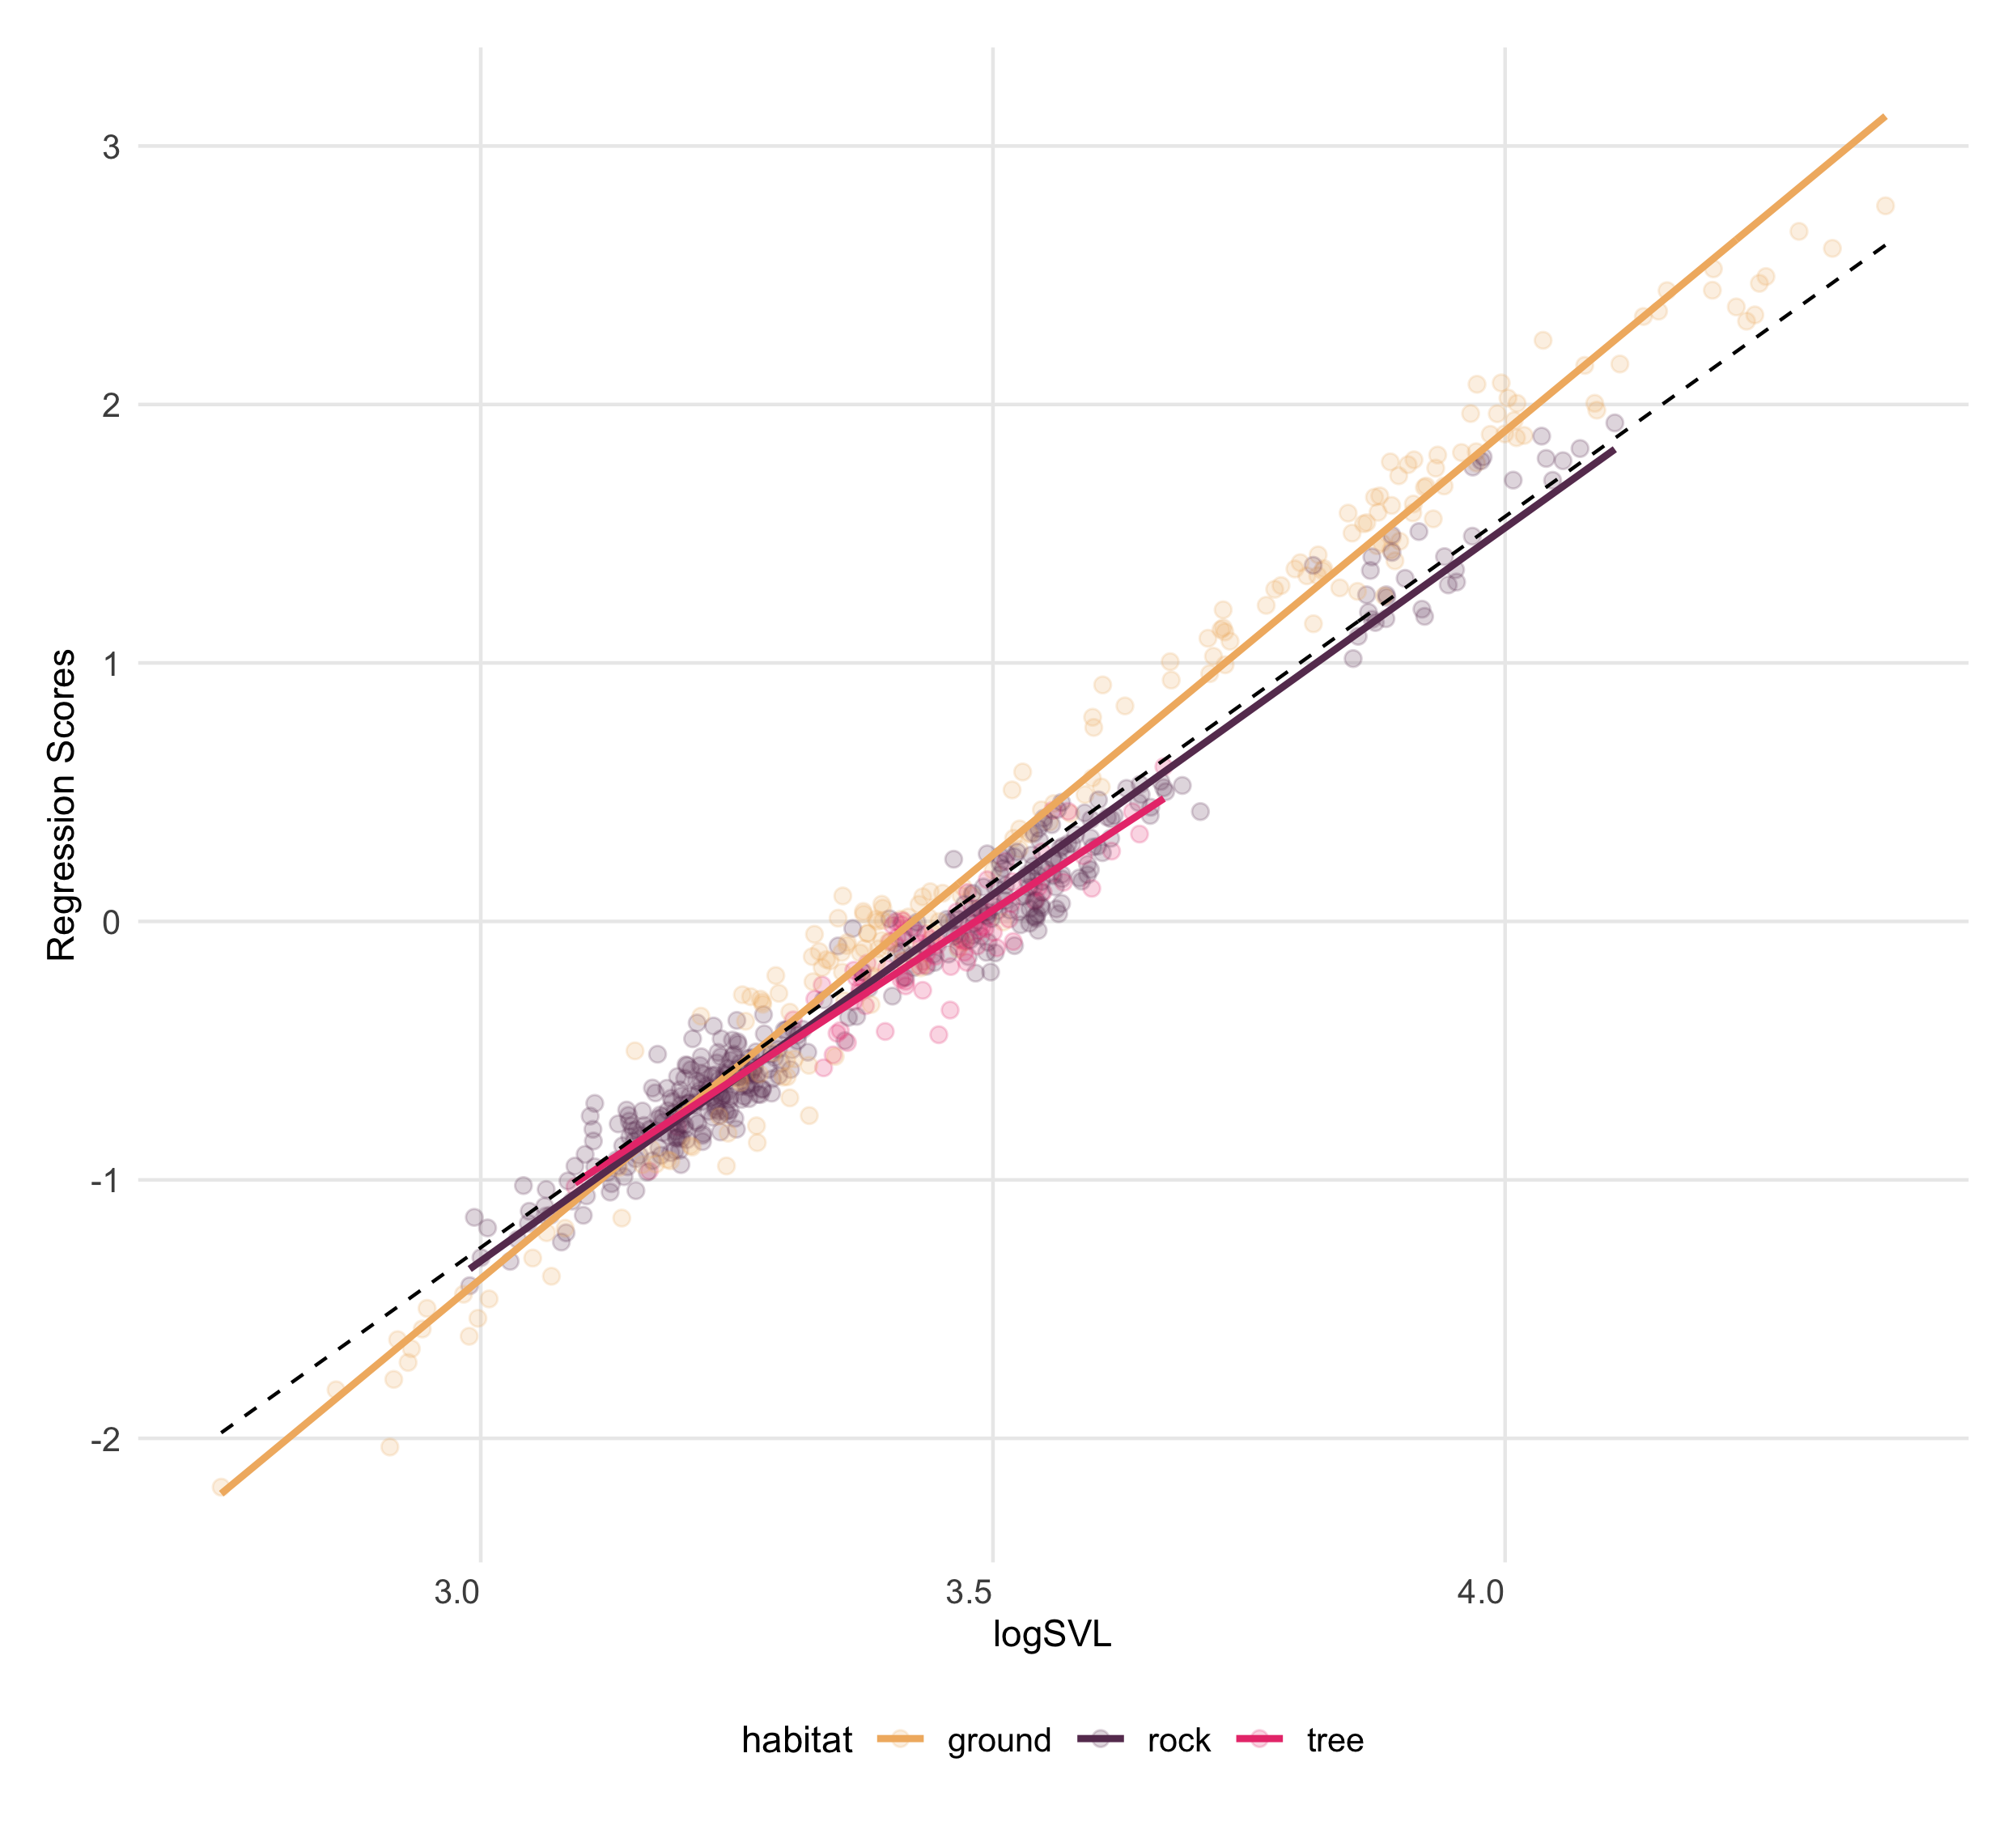
\includegraphics[width=1\linewidth]{Figs/figure_2_ggplot} 

}

\caption{Plot of regression scores and predicted lines representing the relationship between linear body measurements and size (SVL). Individuals are colored by habitat use: ground (beige), rock (dark purple), and tree (magenta). Isometric trend represented by the dashed line.}\label{fig:unnamed-chunk-5}
\end{figure}

\newpage

\begin{figure}

{\centering 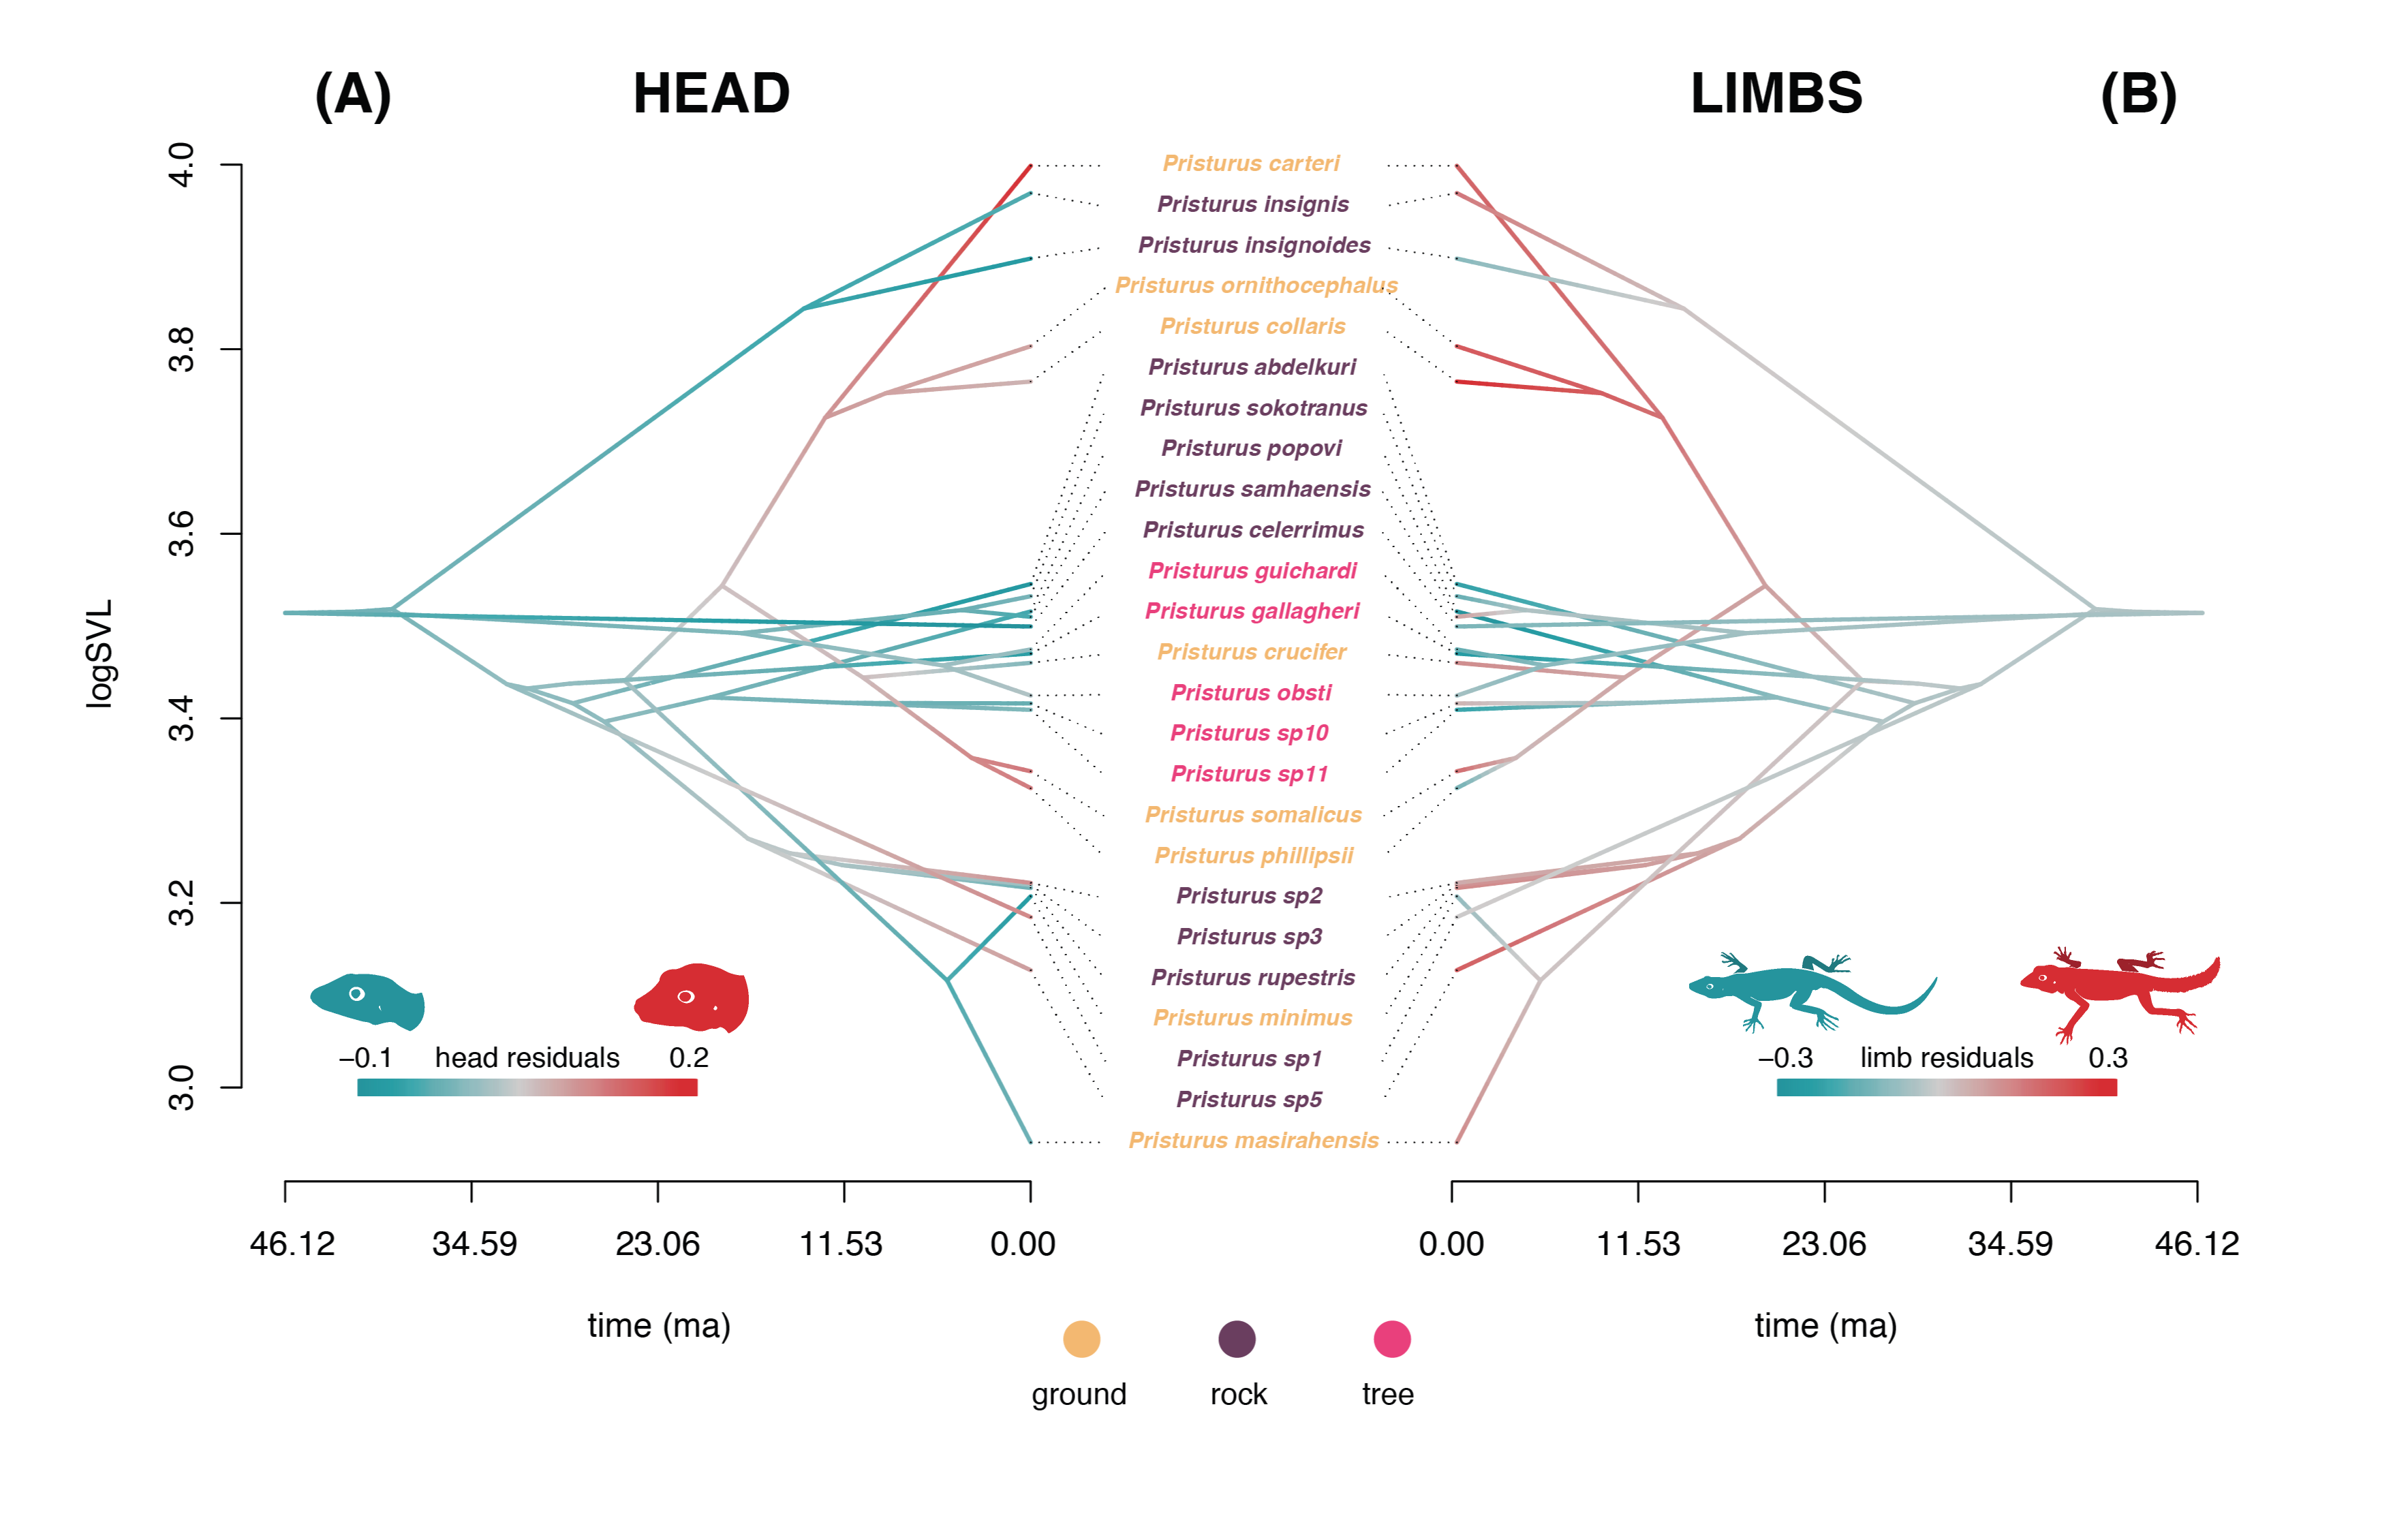
\includegraphics[width=1\linewidth]{Figs/figure_3_Pristurus_allometry_traitgram_legends} 

}

\caption{Traitgrams showing the evolution of body size (SVL) through time based on the phylogenetic tree of \textit{Pristurus}. Colors represent an evolutionary mapping of residuals from phylogenetic regressions describing the relationship of (A) head morphology versus body size, and (B) limb proportions versus body size (see text for descriptions). Species names are colored by habitat use: ground (beige), rock (dark purple), and tree (magenta).}\label{fig:unnamed-chunk-6}
\end{figure}

\newpage

\begin{figure}

{\centering 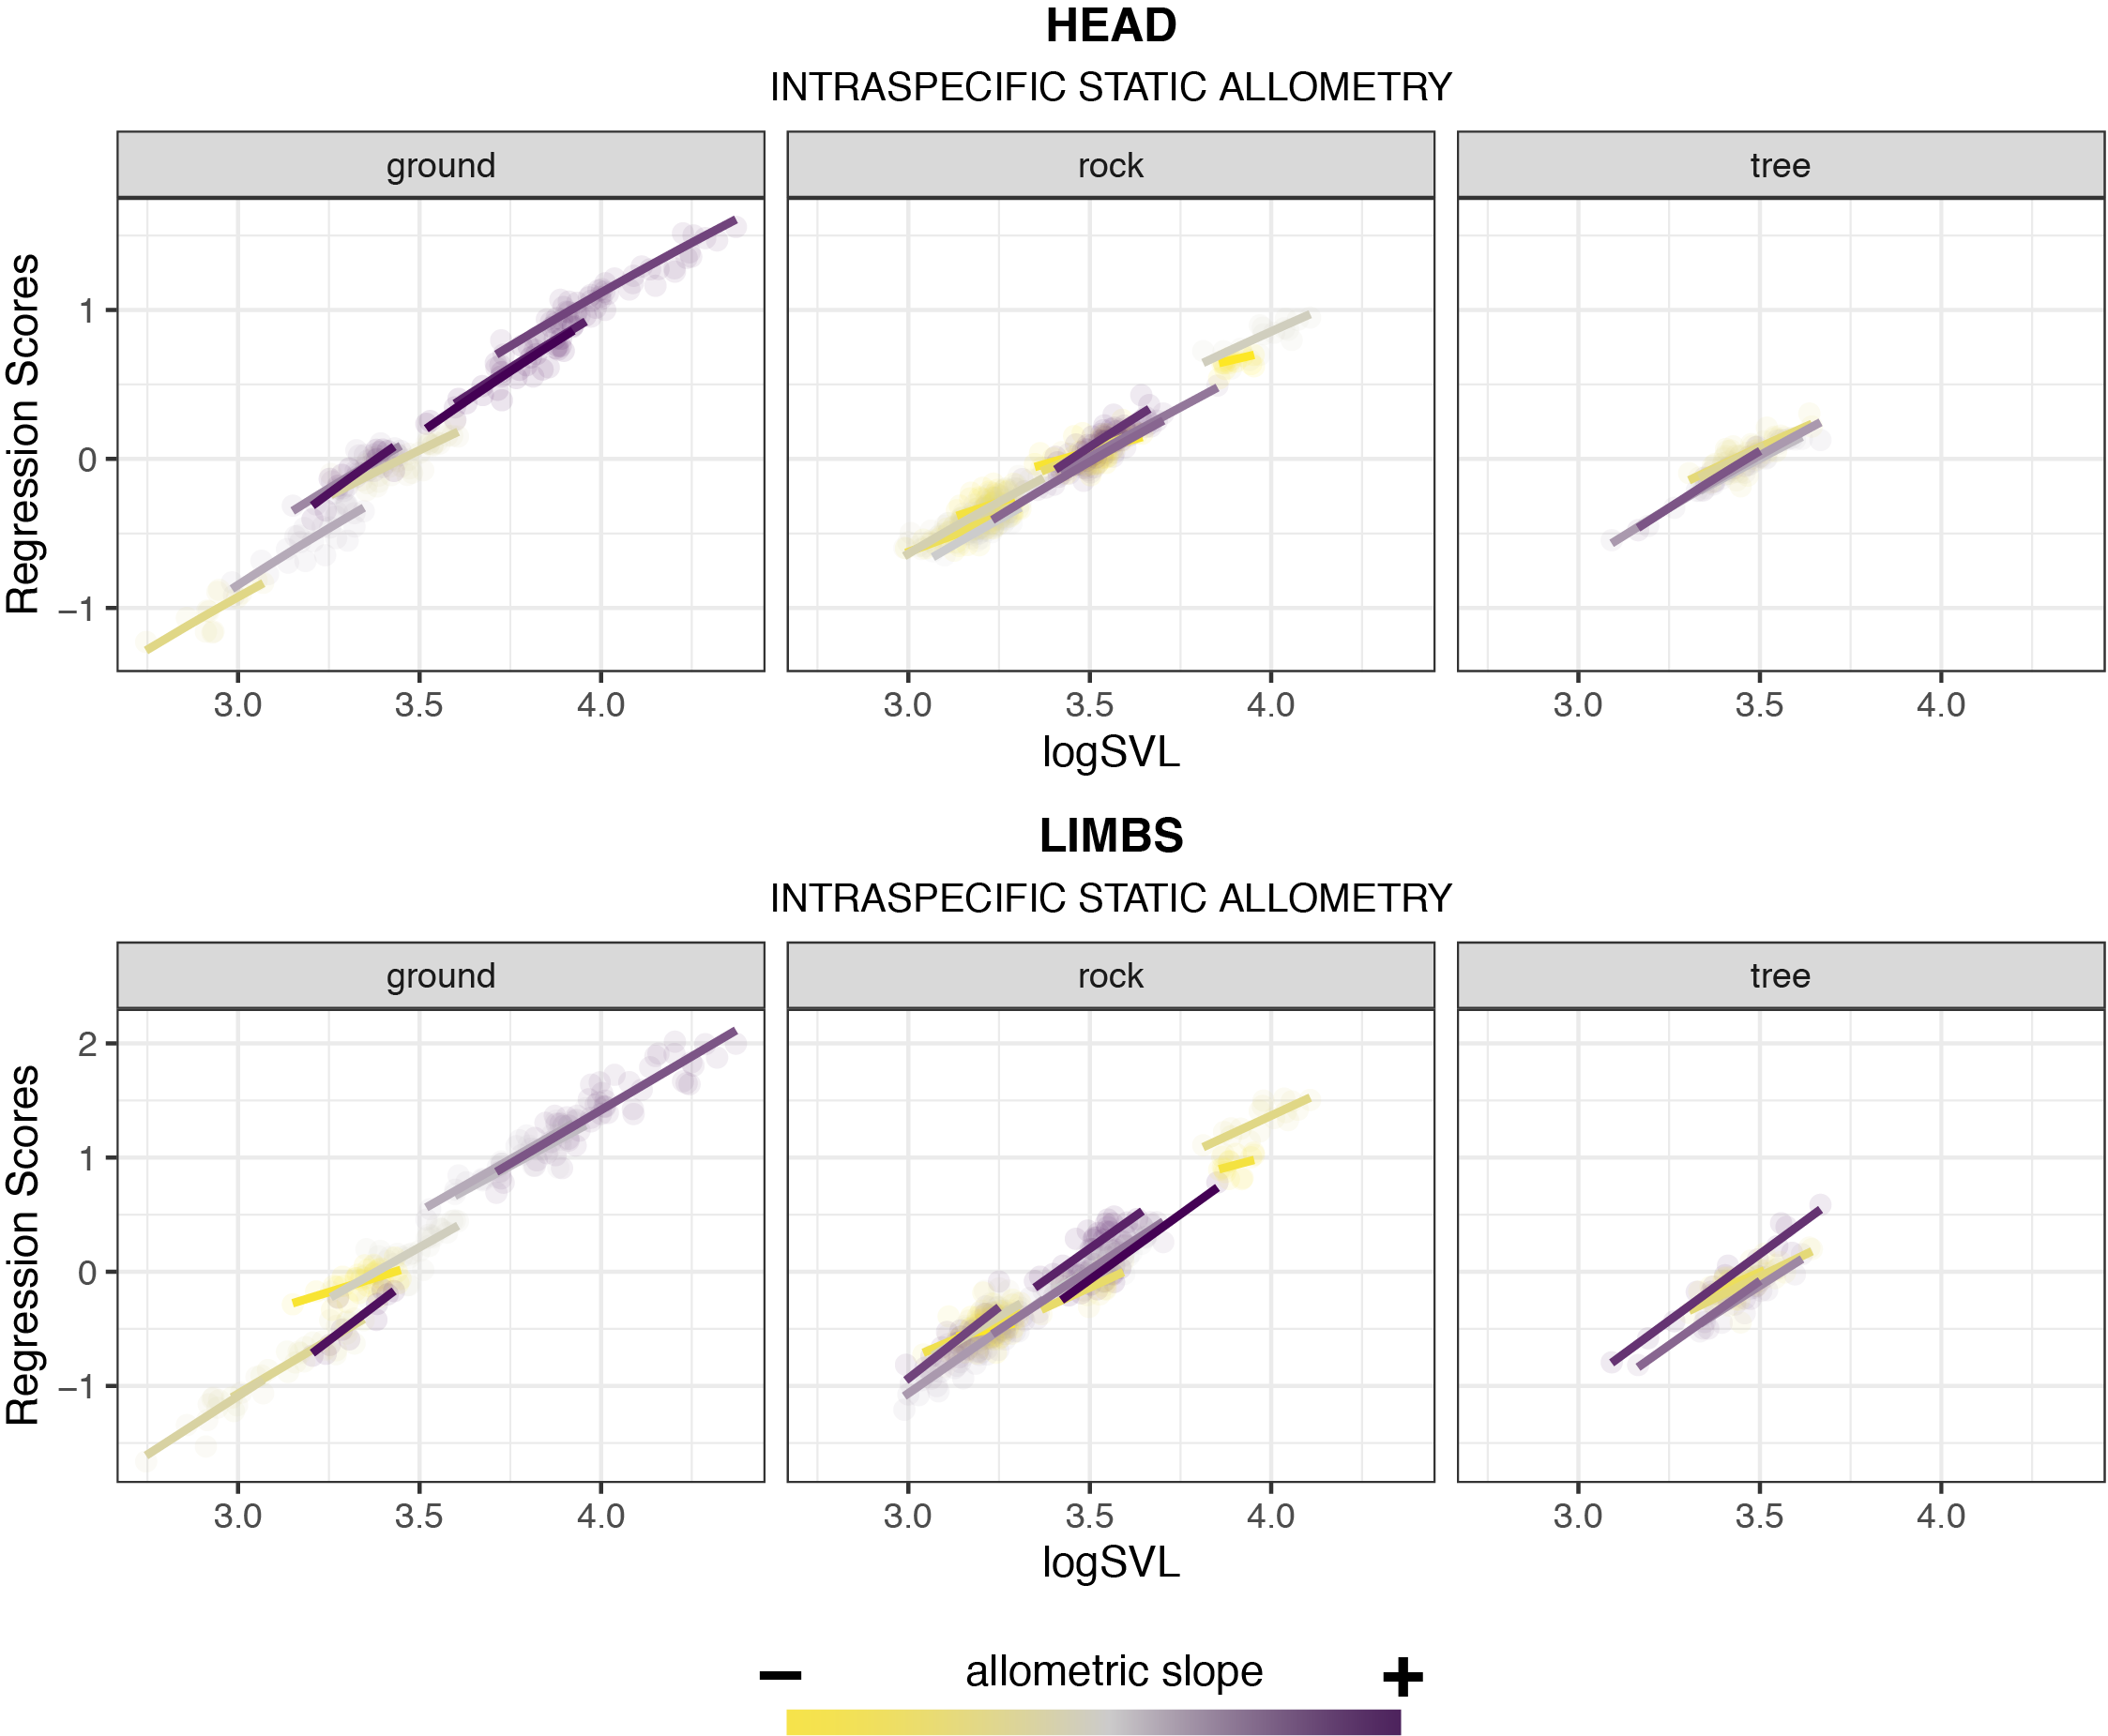
\includegraphics[width=1\linewidth]{Figs/figure_4_static_allometry_v3} 

}

\caption{Patterns of static allometry for each species for head traits (upper panel) and limb traits (lower panel). Species are separated by their habitat groups and colored by the magnitude of their regression slope (purple: steeper slopes, yellow: shallower slopes).}\label{fig:unnamed-chunk-7}
\end{figure}

\newpage

\begin{figure}

{\centering 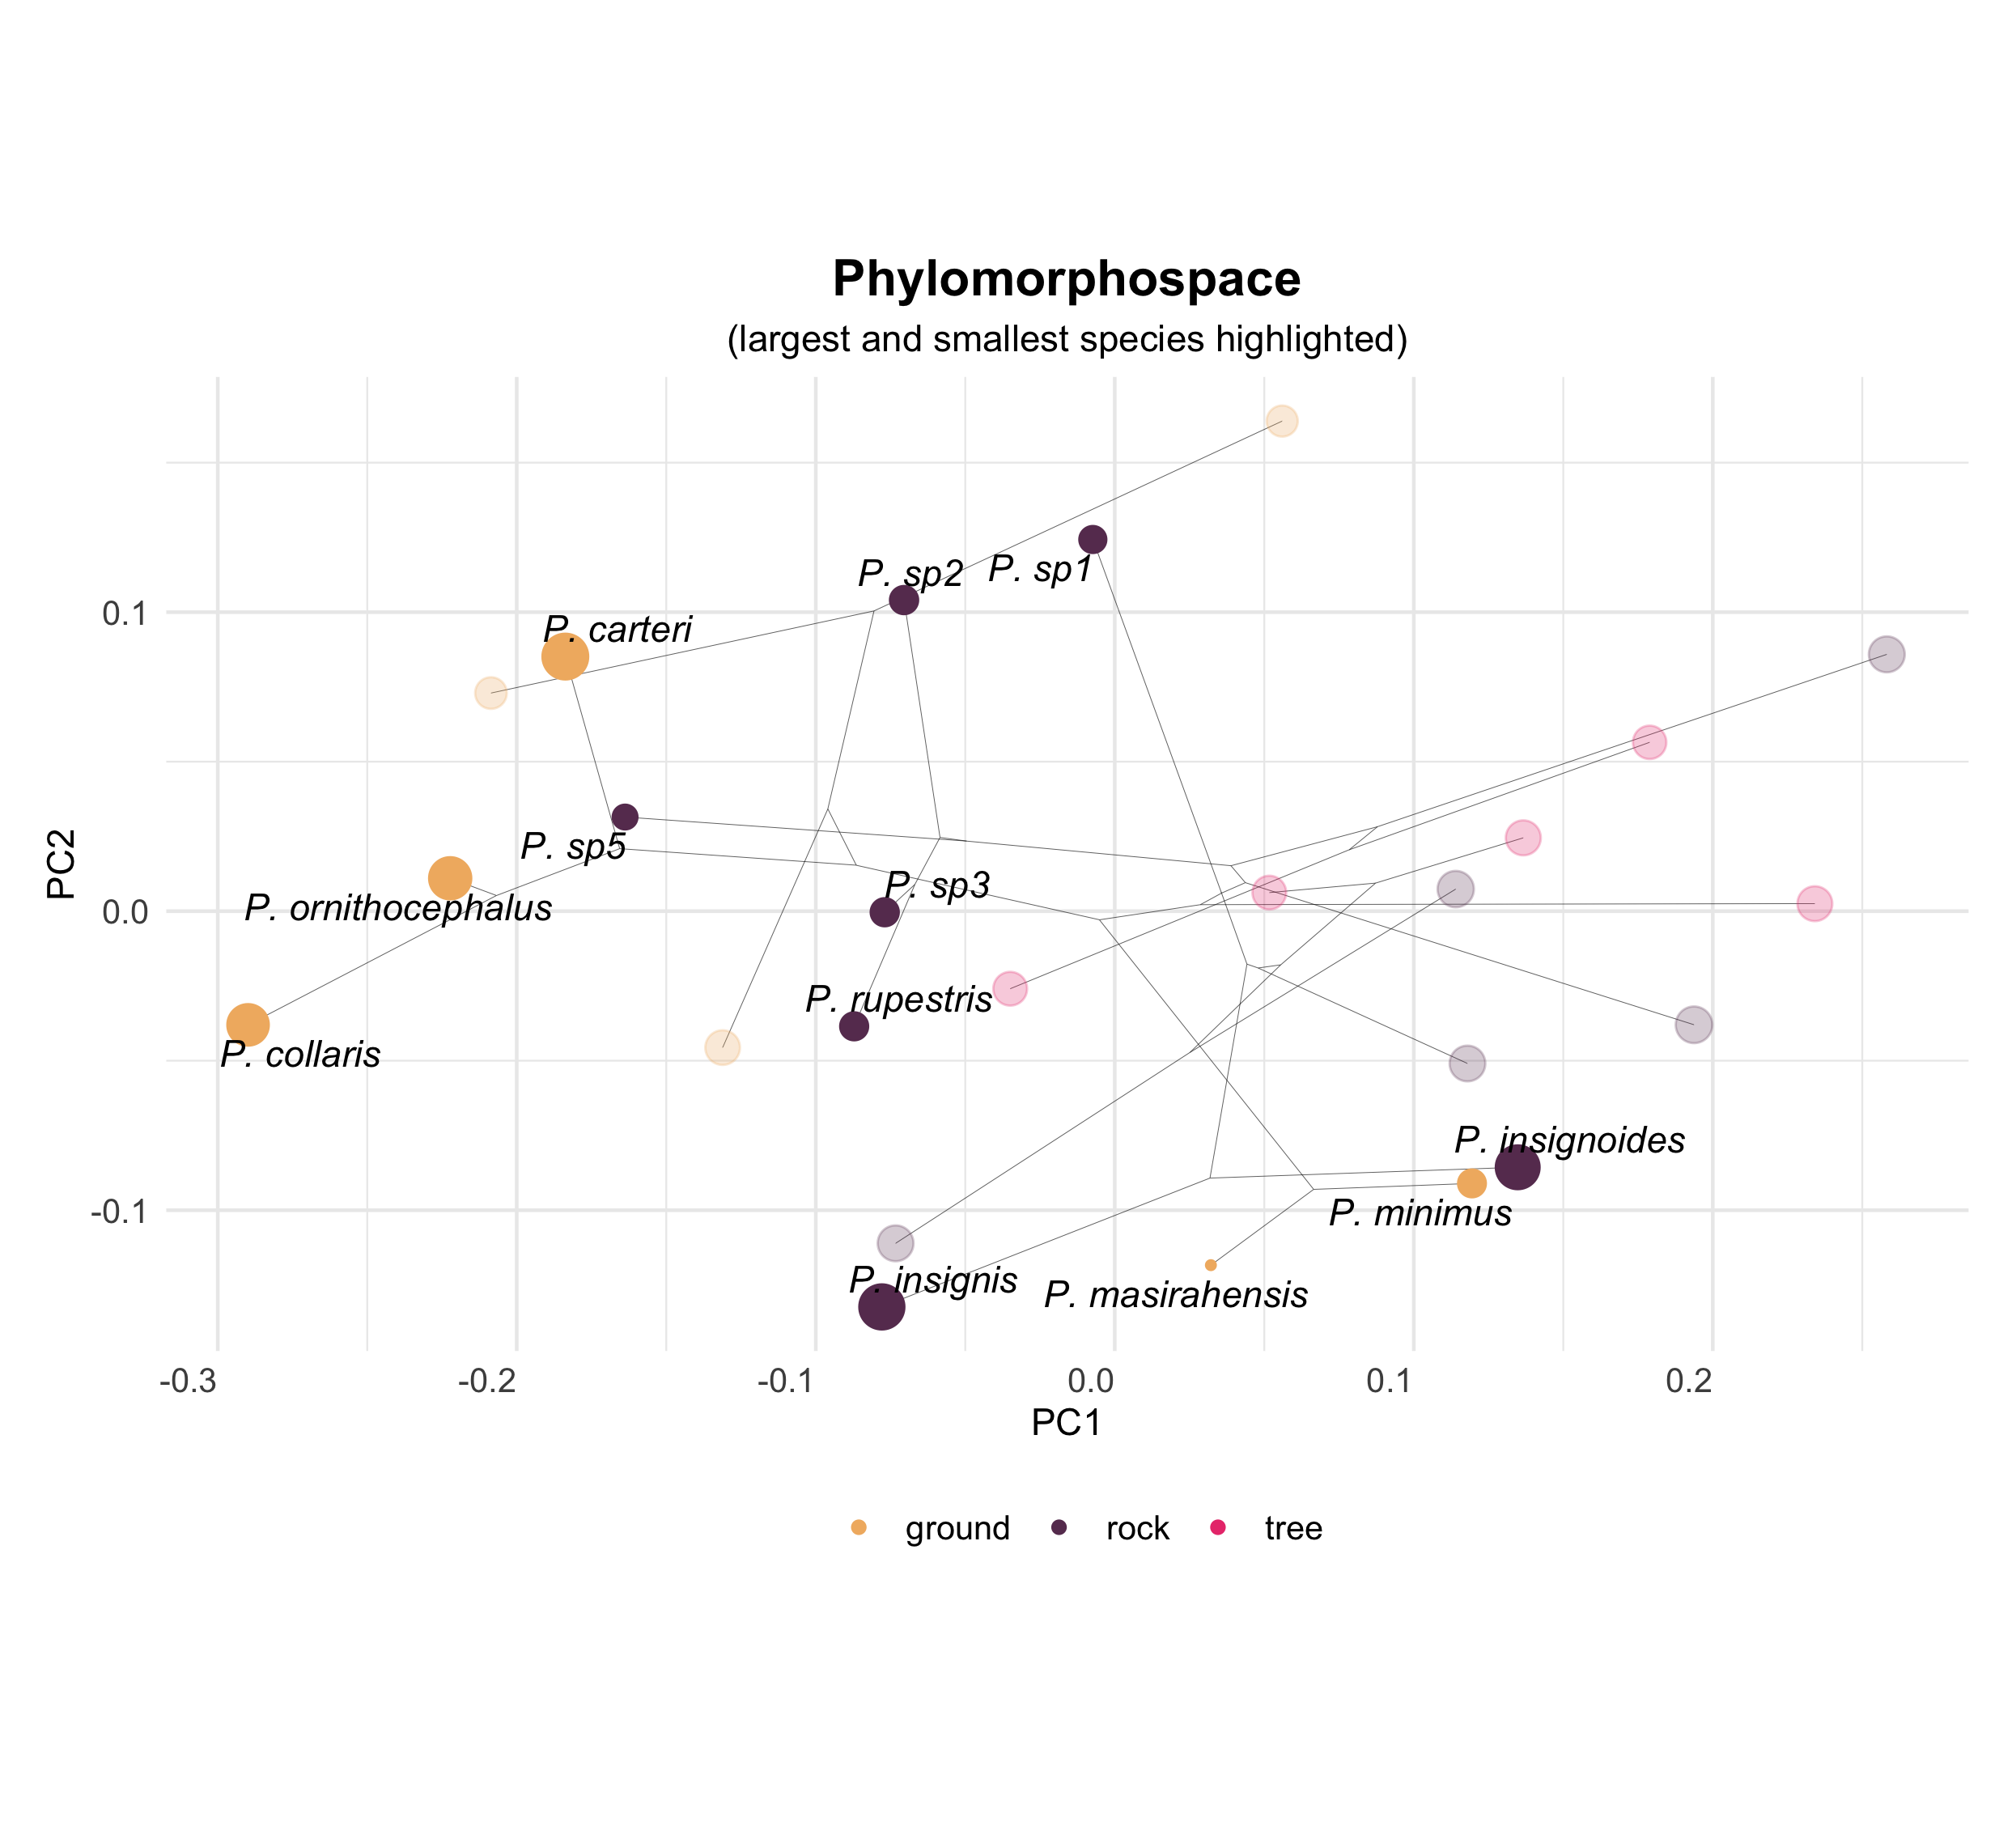
\includegraphics[width=1\linewidth]{Figs/figure_5_phylomorphospace_large_small} 

}

\caption{Phylomorphospace of \textit{Pristurus}, based on residuals from a phylogenetic regression of body measurements on size (SVL). Species means are colored by habitat use: ground (beige), rock (dark purple), and tree (magenta). Large and small rock-dwelling and ground-dwelling are highlighted with darker colors to highlight their differentiation and relative positions in morphospace.}\label{fig:unnamed-chunk-8}
\end{figure}

\newpage

\begin{figure}

{\centering \includegraphics[width=1\linewidth]{Figs/figure_6_Pristurus_allometry_rescaledSVL_horizontal} 

}

\caption{Representative specimens (based on real specimens) from large and small \textit{Pristurus} species, colored by habitat use: ground (beige) and rock (dark purple). Specimens are scaled to a common body size (SVL, gray rectangles) to emphasize the relative differences in limb and head proportions. Relatively slender-headed and short-limbed species shown on the left. Original scale shown as the gray bar.}\label{fig:unnamed-chunk-9}
\end{figure}

\end{document}
